\chapter{Results}
\label{ch:results}

In this chapter the results from the previous in \Autoref{ch:methodology} introduced experiments are presented.
Firstly, \Autoref{ch:results-reproduction} deals with a reproduction and a verification of the results achieved by \textcite{kotelnikov2022TabDDPMModellingTabular}.
Subsequently, \Autoref{ch:results-Metric-results} will present the numerical metric results of the experiments that have been outlined in \Autoref{ch:methodology}.
These include the metric results from the machine learning efficacy scores, as well as the TabSynDex similarity score metrics.
\Autoref{ch:results-Visual} will present selected visual results from the executed experiments, highlighting important characteristics and observations made from the synthetic data that has been generated.
All of this provides the basis for \Autoref{ch:results-discussion}, which analyses and interprets the numerical and visual results from the previous sections.
This section will also revisit and answer the research questions of this thesis from \Autoref{ch:intro-goals} according to the gathered data.
Lastly, this chapter will finish with \Autoref{ch:results-limitations}, critically assessing the constraints and limitations of the study, taking into account the data use, experimental scope, and \gls{model} interpretability.

\section{Reproduction and Verification of Results}
\label{ch:results-reproduction}

Given that this thesis draws heavily upon the research conducted by \cite{kotelnikov2022TabDDPMModellingTabular},
it was deemed necessary to first reproduce the original experiments and subsequently verify the authors' findings,
prior to conducting any new experiments.
Fortunately, the publicly available code \cite{akim2023TabDDPMModellingTabular} facilitated the replication of the experiments with relative ease.

The reproduction is limited to the adult dataset from \Autoref{ch:methods-datasets} and to the machine learning efficacy computed with a tuned CatBoost \cite{prokhorenkova2018CatBoostUnbiasedBoosting} \gls{model}.

Firstly, a CatBoost \gls{model} was tuned on the adult dataset using the provided tuning script (tune\_evaluation\_model.py).
Next, for each sampling algorithm, a \gls{model} was trained according to the configuration files provided by the authors.
Each configuration file contains the parameter settings the authors identified during hyperparameter tuning.
Hence, with the \glspl{model}' respective pipeline.py script, the best-found \gls{model} from hyperparameter tuning could be trained and saved.
Finally, the trained CatBoost and trained sampling \gls{model} were used in the evaluation script (eval\_seeds.py), which calculates and reports the results.

\begin{table}[h]
	\centering
	\begin{tabular}{lccr}
		\toprule
		\textbf{Model}     & \textbf{Reproduction} & \textbf{Original} & \textbf{Difference} \\
		\midrule
		Real               & 0.815                 & 0.815             & 0                   \\
		TVAE$^{ml}$        & 0.780                 & 0.781             & -0.001              \\
		CTABGAN$^{ml}$     & 0.775                 & 0.783             & -0.008              \\
		CTABGAN+$^{ml}$    & 0.775                 & 0.772             & +0.003              \\
		SMOTE$^{ml}$       & 0.791                 & 0.791             & 0                   \\
		TabDDPM$^{ml}_{q}$ & 0.794                 & 0.795             & -0.001              \\
		\bottomrule
		\multicolumn{4}{c}{}\\[-0.6em]
	\end{tabular}
	\caption[Reproduction Original Results]{Comparison of the CatBoost F1-score on synthetic datasets created by different sampling \glspl{model}.
		F1-Scores of the reproduction experiments are compared against the results reported by the original authors \cite[Table 4, p. 8]{kotelnikov2022TabDDPMModellingTabular}.}
	\label{tab:reproduction}
\end{table}

\Autoref{tab:reproduction} shows the computed F1-scores achieved by the CatBoost \gls{model} when trained on different synthetic datasets generated by different sampling \glspl{model}.
The scores that could be reproduced are almost exactly the same as those reported by the original authors.
All differences are within the standard deviation reported by the authors, except for the CTABGAN \gls{model}.
It is unclear why the CTABGAN \gls{model} score deviates in the reproduction experiment from the original score.
However, it is important to note that minor modifications to the code or different Python library versions could have caused this alternation, which were required to train the \gls{model} in the cloud environment, specified in \Autoref{ch:methods-experimentalSetup}.
Nevertheless, the reproduced score for the CTABGAN \gls{model} is still very close to the original score.
Hence, the overall outcome reported by the authors was successfully replicated and confirmed.

\section{Metric Results}
\label{ch:results-Metric-results}

\Autoref{ch:results-Metric-results} delves into the metric results of the conducted research. 
The chapter starts with baseline experiments in \Autoref{ch:Baseline}, which provides a reference point for the subsequent modifications. 
\Autoref{ch:Experiment-1} presents the first experimental changes with the incorporation of tabular processing. 
In \Autoref{ch:Experiment-2}, the focus shifts to the effects of changing the hyperparameters strategy.
Finally, \Autoref{ch:Experiment-3} details the third set of experiments, exploring to what extent a change in the normalization process affected the metric results. 
The chapter's objective is to highlight and compare the results of these experimental variations.

\subsection{Baseline Experiments}
\label{ch:Baseline}

After verifying that the \glspl{model} are able to reproduce the machine-learning efficacy scores as reported,
their performance is additionally evaluated using the similarity evaluation as proposed in \Autoref{ch:conceptualDesign-Evaluation}.
\Autoref{tab:ml_baseline} shows the complete machine learning efficacy score results for the different sampling techniques:

\begin{table}[h]
	\centering
	\begin{tabular}{lccr}
		\toprule
		\textbf{Model}     & \textbf{Accuracy} & \textbf{F1}    & \textbf{ROC-AUC} \\
		\midrule
		Real               & 0.874              & 0.815          & 0.928            \\
		TVAE$^{ml}$        & 0.845              & 0.780          & 0.900            \\
		CTABGAN$^{ml}$     & 0.850              & 0.775          & 0.900            \\
		CTABGAN+$^{ml}$    & 0.855              & 0.775          & 0.907            \\
		SMOTE$^{ml}$       & 0.858              & 0.791          & 0.910            \\
		TabDDPM$^{ml}_{q}$ & \textbf{0.860}     & \textbf{0.794} & \textbf{0.913}   \\
		\bottomrule
		\multicolumn{4}{c}{}\\[-0.6em]
	\end{tabular}
	\caption[ML Efficacy Baseline]{Machine learning efficacy (CatBoost) baseline results. The best results are highlighted in bold (excluding the real data).}
	\label{tab:ml_baseline}
\end{table}


In addition to the machine learning efficacy scores, the similarity scores of the TabSynDex metric (compare \Autoref{ch:preliminaries-similarityScore}) are computed (\Autoref{tab:sim_baseline}).

\begin{table}[h]
	\centering
	\begin{tabular}{lrrrrrr}
		\toprule
		\textbf{Model}     & \textbf{Similarity Score} & \textbf{Basic} & \textbf{Correlation} & \textbf{ML}    & \textbf{Support} & \textbf{pMSE}  \\
		\midrule
		Real               & 0.960                     & 0.992          & 0.943                & 0.998          & 0.984            & 0.882          \\
		TVAE$^{ml}$        & 0.658                     & 0.854          & 0.814                & 0.962          & 0.657            & 0.000          \\
		CTABGAN$^{ml}$     & 0.741                     & 0.940          & 0.832                & 0.984          & \textbf{0.947}   & 0.000          \\
		CTABGAN+$^{ml}$    & 0.750                     & 0.969          & 0.882                & 0.990          & 0.892            & 0.019          \\
		SMOTE$^{ml}$       & 0.723                     & 0.953          & 0.865                & \textbf{0.992} & 0.804            & 0.000          \\
		TabDDPM$^{ml}_{q}$ & \textbf{0.759}            & \textbf{0.973} & \textbf{0.919}       & \textbf{0.992} & 0.874            & \textbf{0.035} \\
		\bottomrule
		\multicolumn{7}{c}{}\\[-0.6em]
	\end{tabular}
	\caption[TabSynDex Baseline]{Similarity baseline results using the TabSynDex metrics. The \textit{similarity score} is the average of the other five scores. The best results are highlighted in bold.}
	\label{tab:sim_baseline}
\end{table}

These baseline experiments show that the diffusion-based synthesis approach outperforms other \glspl{model} not only in terms of machine learning efficacy but also in terms of other metrics.
However, \Autoref{tab:sim_baseline} shows that the CTABGAN \glspl{model} outperform TabDDPM in the support coverage metric.
Additionally, it is worth mentioning that even though TabDDPM achieves the highest \gls{pmse} score, it is still extremely low and almost 0, which is the same for all other \glspl{model}.
The authors of \cite{chundawat2022UniversalMetricRobust} confirm this observation in their experiments.
During their experiments, the tested sampling techniques (various \gls{gan}-based approaches) also struggle to produce any synthetic data which achieves a \gls{pmse} score that is noticeably higher than 0.
\Autoref{tab:sim_baseline} indicates that this observation also holds for a diffusion-based approach, whose hyperparameters were tuned towards a machine learning efficacy score using a CatBoost \gls{model}.

\subsection{Experiment 1: Adding Tabular Processing}
\label{ch:Experiment-1}

The first set of experiments evaluates the different tabular processing mechanisms described in \Autoref{ch:architecture-tabularProcessor-implementations}.
For this, the tabular processing mechanisms have been added to the pipeline of TabDDPM, as described in the concept in \Autoref{fig:Overall_changed}.
Consequently, the diffusion \gls{model}'s tuning (tune\_ddpm.py, see \Autoref{ch:scripts}) with the additional tabular processing was required.
The \glspl{model}' hyperparameters have again been tuned towards the machine learning efficacy of a CatBoost \gls{model}.

\begin{table}[h]
	\centering
	\begin{tabular}{lrrr}
		\toprule
		\textbf{Model}         & \textbf{Accuracy} & \textbf{F1}    & \textbf{ROC-AUC} \\
		\midrule
		Real                   & 0.874              & 0.815          & 0.928            \\
		TabDDPM$^{ml}_{q}$     & 0.860              & 0.794          & 0.913            \\
		TabDDPM-BGM$^{ml}_{q}$ & \textbf{0.863}     & \textbf{0.798} & \textbf{0.916}   \\
		TabDDPM-FT$^{ml}_{q}$  & 0.785              & 0.552          & 0.821            \\
		\bottomrule
		\multicolumn{4}{c}{}\\[-0.6em]
	\end{tabular}
	\caption[Experiment 1 ML efficacy]{CatBoost machine learning efficacy scores for different tabular processing techniques.}
	\label{tab:exp1-ml}
\end{table}

\begin{table}[h]
	\centering
	\begin{tabular}{lrrrrrr}
		\toprule
		\textbf{Model}         & \textbf{Similarity Score} & \textbf{Basic} & \textbf{Correlation} & \textbf{ML}    & \textbf{Support} & \textbf{pMSE}  \\
		\midrule
		Real                   & 0.960                     & 0.992          & 0.943                & 0.998          & 0.984            & 0.882          \\
		TabDDPM$^{ml}_{q}$     & \textbf{0.759}            & \textbf{0.973} & \textbf{0.919}       & 0.992          & 0.874            & \textbf{0.035} \\
		TabDDPM-BGM$^{ml}_{q}$ & 0.742                     & 0.964          & 0.918                & \textbf{0.996} & 0.831            & 0.000          \\
		TabDDPM-FT$^{ml}_{q}$  & 0.595                     & 0.495          & 0.648                & 0.869          & \textbf{0.963}   & 0.000          \\
		\bottomrule
		\multicolumn{7}{c}{}\\[-0.6em]
	\end{tabular}
	\caption[Experiment 1 TabSynDex]{TabSynDex evaluation metric scores for different tabular processing techniques.}
	\label{tab:exp1-sim}
\end{table}

The results of the machine learning efficacy and TabSynDex metric results can be found in \Autoref{tab:exp1-ml} and \Autoref{tab:exp1-sim}, respectively.
Both evaluations show that the additional \gls{bgm} tabular processing increases the machine learning efficacy scores.
All metrics in \Autoref{tab:exp1-ml} are highest for the TabDDPM-BGM \gls{model} and the machine learning efficacy score of TabSynDex (which makes use of different machine learning \glspl{model})
is highest for TabDDPM-BGM as well, although only by a slight margin.
\Autoref{tab:exp1-sim} indicates that this increase seems to come at the cost of reduced performance in the other metrics, which are highest for the basic, correlation and \gls{pmse} metric scores for the plain TabDDPM version.
The performance of TabDDPM-FT lags notably behind its counterparts in terms of correlation and basic metric scores.
Interestingly, TabDDPM-FT performance is significantly better in the support score than the other versions and approximately 13\%-points worse in terms of the machine learning efficacy score computed by the TabSynDex metric.
More details can be seen in the \Autoref{tab:exp1-ml}, which shows that especially the F1 score from TabDDPM-FT is much worse than the F1 score of the other \glspl{model}.
Lastly, neither the \gls{bgm} nor the \gls{ft} tabular processing enable the diffusion \gls{model} to produce synthetic data that is able to increase the \gls{pmse} score.


\subsection{Experiment 2: Similarity Hyperparameter Optimization}
\label{ch:Experiment-2}

The second set of experiments is very similar to the first experiment.
Instead of tuning the \glspl{model}' hyperparameters after the machine learning efficacy, as proposed by the original authors,
the \glspl{model}' hyperparameters are tuned after the TabSynDex similarity score.

The machine learning efficacy and TabSynDex metric results can be found in \Autoref{tab:exp2-ml} and \Autoref{tab:exp2-sim}, respectively.



\begin{table}[h]
	\centering
	\begin{tabular}{lrrr}
		\toprule
		\textbf{Model}        & \textbf{Accuracy} & \textbf{F1}    & \textbf{ROC-AUC} \\
		\midrule
		Real                  & 0.874              & 0.815          & 0.928            \\
		TabDDPM$^{s}_{q}$     & 0.856              & 0.782          & 0.908            \\
		TabDDPM-BGM$^{s}_{q}$ & \textbf{0.859}     & \textbf{0.792} & \textbf{0.911}   \\
		TabDDPM-FT$^{s}_{q}$  & 0.767              & 0.450          & 0.712            \\
		CTABGAN$^{s}$         & 0.850              & 0.776          & 0.900            \\
		CTABGAN+$^{s}$        & 0.851              & 0.768          & 0.902            \\
		TVAE$^{s}$            & 0.845              & 0.780          & 0.900            \\
		\bottomrule
		\multicolumn{4}{c}{}\\[-0.6em]
	\end{tabular}
	\caption[Experiment 2 ML efficacy]{CatBoost machine learning efficacy scores for different tabular processing techniques, whose hyperparameters have been tuned towards the TabSynDex similarity score.}
	\label{tab:exp2-ml}
\end{table}

\begin{table}[h]
	\centering
	\begin{tabular}{lrrrrrr}
		\toprule
		\textbf{Model}        & \textbf{Similarity Score} & \textbf{Basic} & \textbf{Correlation} & \textbf{ML}    & \textbf{Support} & \textbf{pMSE}  \\
		\midrule
		Real                  & 0.960                     & 0.992          & 0.943                & 0.998          & 0.984            & 0.882          \\
		TabDDPM$^{s}_{q}$     & 0.852                     & 0.976          & \textbf{0.921}       & \textbf{0.991} & 0.952            & 0.420          \\
		TabDDPM-BGM$^{s}_{q}$ & \textbf{0.857}            & \textbf{0.982} & 0.858                & \textbf{0.991} & 0.920            & \textbf{0.532} \\
		TabDDPM-FT$^{s}_{q}$  & 0.589                     & 0.513          & 0.620                & 0.819          & \textbf{0.992}   & 0.000          \\
		CTABGAN$^{s}$         & 0.740                     & 0.938          & 0.833                & 0.984          & 0.947            & 0.000          \\
		CTABGAN+$^{s}$        & 0.784                     & 0.970          & 0.888                & 0.987          & 0.908            & 0.167          \\
		TVAE$^{s}$            & 0.658                     & 0.856          & 0.815                & 0.962          & 0.656            & 0.000          \\
		\bottomrule
		\multicolumn{7}{c}{}\\[-0.6em]
	\end{tabular}
	\caption[Experiment 2 TabSynDex]{TabSynDex evaluation metric scores for different tabular processing techniques, whose hyperparameters have been tuned towards the TabSynDex similarity score.}
	\label{tab:exp2-sim}
\end{table}

The results show that TabDDPM-BGM outperforms all other \glspl{model} in terms of the CatBoost machine learning efficacy and is on par with TabDDPM in the TabSynDex machine learning efficacy score.
TabDDPM-BGM also has the highest overall similarity score and achieves the highest basic and \gls{pmse} metric scores.
However, the simpler TabDDPM outperforms its \gls{bgm} counterpart regarding the correlation and support metric scores.
Overall, TabDDPM achieves comparable performance to TabDDPM-BGM on all metrics, with the biggest difference in the \gls{pmse} score of -0.11\%-points.
TabDDPM-FT performance is significantly worse than all other TabDDPM variants in all metrics except the support score.
On the one hand, it seems to be the case that hyperparameter tuning after the similarity score does have a big influence on the TabDDPM and TabDDPM-BGM \glspl{model}' \gls{pmse} score.
On the other hand, this hyperparameter tuning did not affect the \gls{pmse} score of the other tested \glspl{model}, the CTABGAN, TVAE, or the TabDDPM-FT, all having zero \gls{pmse} scores.
The CTABGAN+$^{s}$ \gls{model} is the only non-diffusion \gls{model} that achieves a non-zero \gls{pmse} score of 0.167\%, which is still noticeably smaller than the score of TabDDPM$^{s}_{q}$ and TabDDPM-BGM$^{s}_{q}$.
\newpage
\subsection{Experiment 3: Exchanging the Normalization}
\label{ch:Experiment-3}

So far, all TabDDPM \glspl{model} received data normalized according to the quantile transform function (applied after tabular processing), as proposed in \cite{kotelnikov2022TabDDPMModellingTabular}.
A third experiment will investigate how the \glspl{model} perform when their quantile transform function is replaced by a simpler min-max scaler, as explained in \Autoref{sec:dataNormalization}.
Based upon the performance of the \gls{model} variants so far, only the plain TabDDPM and TabDDPM-BGM, tuned after the similarity score will be investigated since the performance of
TabDDPM-FT was noticeably worse.

\begin{table}[h]
	\centering
	\begin{tabular}{lrrr}
		\toprule
		\textbf{Model}        & \textbf{Accuracy} & \textbf{F1}    & \textbf{ROC-AUC} \\
		\midrule
		Real                  & 0.874              & 0.815          & 0.928            \\
		TabDDPM$^{s}_{m}$     & 0.856              & 0.778          & \textbf{0.910}   \\
		TabDDPM-BGM$^{s}_{m}$ & \textbf{0.857}     & \textbf{0.787} & 0.909            \\
		TabDDPM-BGM$^{s}_{n}$ & 0.855              & 0.784          & 0.907            \\
		\bottomrule
		\multicolumn{4}{c}{}\\[-0.6em]
	\end{tabular}
	\caption[Experiment 3 ML efficacy]{CatBoost Machine learning efficacy scores for different tabular processing techniques whose hyperparameters have been tuned towards the TabSynDex similarity score
		and the data was transformed according to a min-max-scaler.}
	\label{tab:exp3-ml}
\end{table}

\begin{table}[h]
	\centering
	\begin{tabular}{lrrrrrr}
		\toprule
		\textbf{Model}        & \textbf{Similarity Score} & \textbf{Basic} & \textbf{Correlation} & \textbf{ML}    & \textbf{Support} & \textbf{pMSE}  \\
		\midrule
		Real                  & 0.960                     & 0.992          & 0.943                & 0.998          & 0.984            & 0.882          \\
		TabDDPM$^{s}_{m}$     & \textbf{0.869}            & 0.938          & \textbf{0.930}       & 0.990          & \textbf{0.928}   & \textbf{0.558} \\
		TabDDPM-BGM$^{s}_{m}$ & 0.856                     & \textbf{0.981} & 0.913                & \textbf{0.992} & 0.915            & 0.476          \\
		TabDDPM-BGM$^{s}_{n}$ & 0.833                     & 0.975          & 0.916                & \textbf{0.992} & 0.915            & 0.369          \\
		\bottomrule
		\multicolumn{7}{c}{}\\[-0.6em]
	\end{tabular}
	\caption[Experiment 3 TabSynDex]{TabSynDex evaluation metric scores for different tabular processing techniques whose hyperparameters have been tuned towards the TabSynDex similarity score
		and the data was transformed according to a min-max-scaler.}
	\label{tab:exp3-sim}
\end{table}

Given the results in \Autoref{tab:exp3-ml} and \Autoref{tab:exp3-sim}, it seems to be the case that TabDDPM-BGM outperforms TabDDPM in terms of the TabSynDex machine learning efficacy and the basic metric scores, but only by a slight margin.
TabDDPM, on the other hand, achieves a higher overall similarity score, mainly due to the superior performance in the correlation, support, and \gls{pmse} scores.
Additionally, not having any transformation after the tabular processing (TabDDPM-BGM$^{s}_{n}$) results in an overall slightly worse similarity score compared to applying a min-max transformation.
\newpage
\section{Visual Results}
\label{ch:results-Visual}

Several plots have been produced according to the methodology of \cite{brenninkmeijer2019GenerationEvaluationTabular}.
This section will cover which plots have been produced and how the plots for different \gls{model} versions differ.

\subsection{Correlation Difference Matrix}

Correlation matrices have been computed to get an intuition on how well correlations between two variables within the dataset are reproduced.
The correlation matrix for the synthetic dataset has been subtracted from the correlation matrix of the real dataset in order to produce a correlation difference matrix.
The smaller the difference, the more similar the correlations within the synthetic dataset are to the correlations within the real dataset.

Looking at the correlations matrix differences in \Autoref{fig:corr_base} for the baseline \glspl{model} that are not diffusion-based, one can see that the CTABGAN+$^{ml}$ and \gls{smote} approaches have the smallest
correlation matrix difference.
However, the diffusion \gls{model} TabDDPM$^{ml}$ produces the matrix with the smallest overall differences.

\begin{figure}[h]
	\centering
	\begin{subfigure}{0.3\textwidth}
		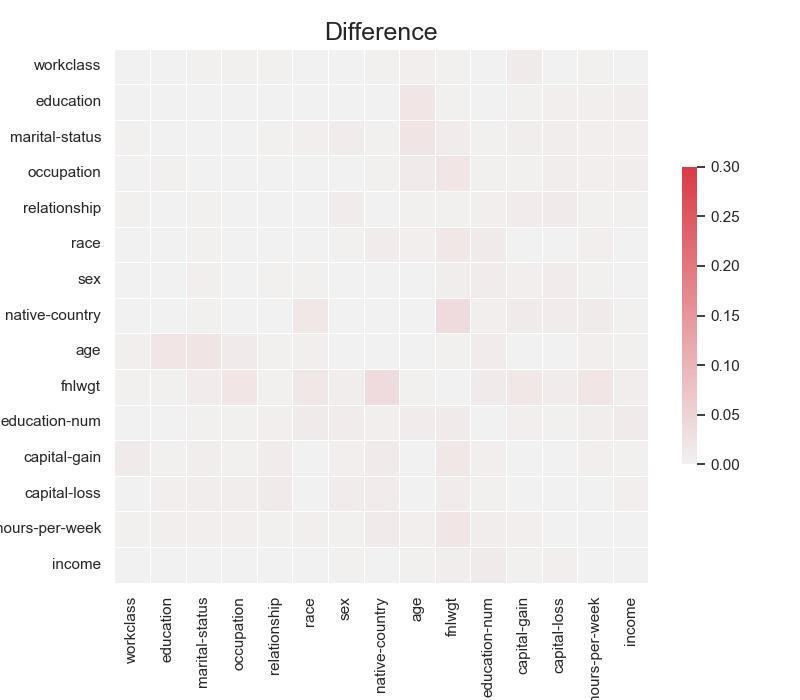
\includegraphics[width=\textwidth]{images/correlation_difference/real.jpg}
		\caption{Real}

	\end{subfigure}
	\hfill
	\begin{subfigure}{0.3\textwidth}
		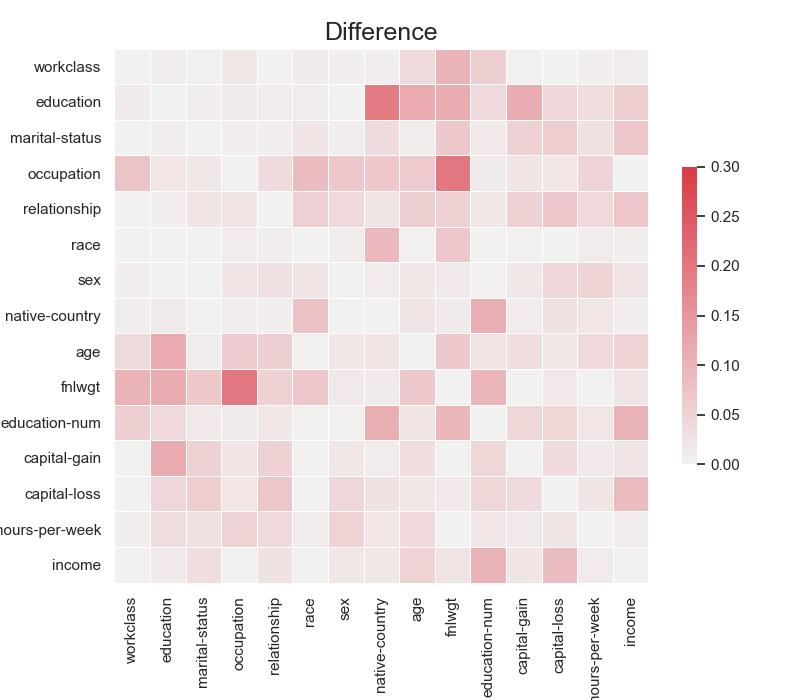
\includegraphics[width=\textwidth]{images/correlation_difference/tvae.jpg}
		\caption{TVAE$^{ml}$}

	\end{subfigure}
	\hfill
	\begin{subfigure}{0.3\textwidth}
		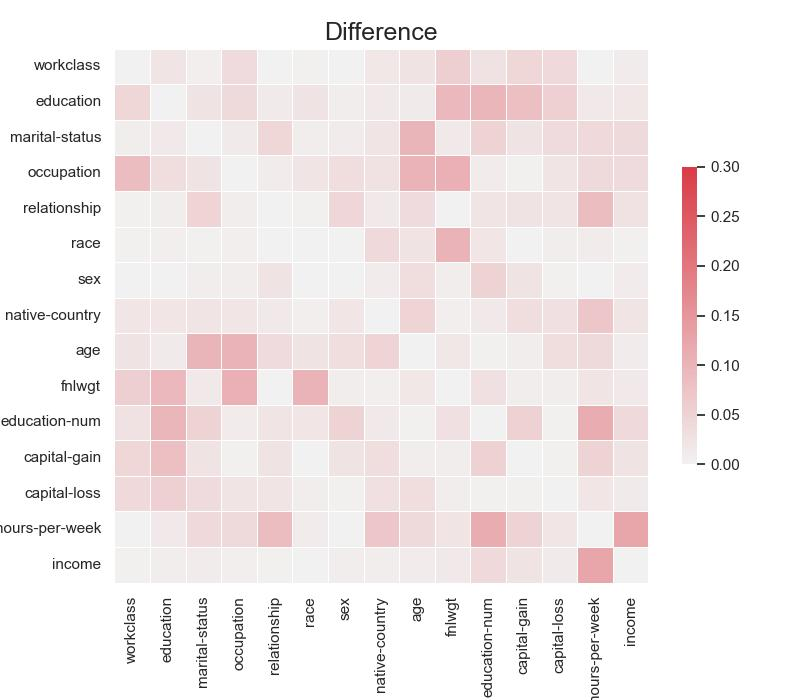
\includegraphics[width=\textwidth]{images/correlation_difference/ctabgan.jpg}
		\caption{CTABGAN$^{ml}$}
	\end{subfigure}

	\begin{subfigure}{0.3\textwidth}
		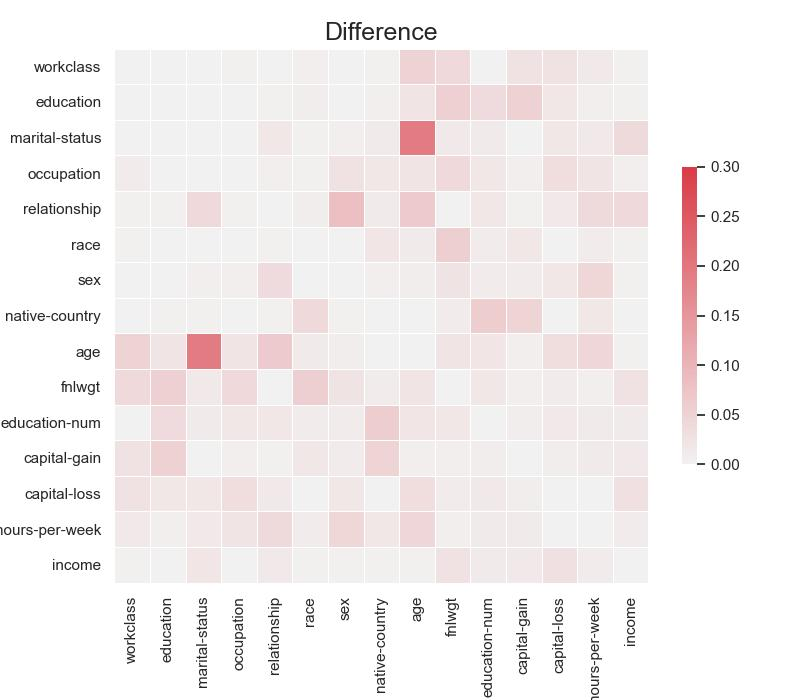
\includegraphics[width=\textwidth]{images/correlation_difference/ctabgan+.jpg}
		\caption{CTABGAN+$^{ml}$}

	\end{subfigure}
	\begin{subfigure}{0.3\textwidth}
		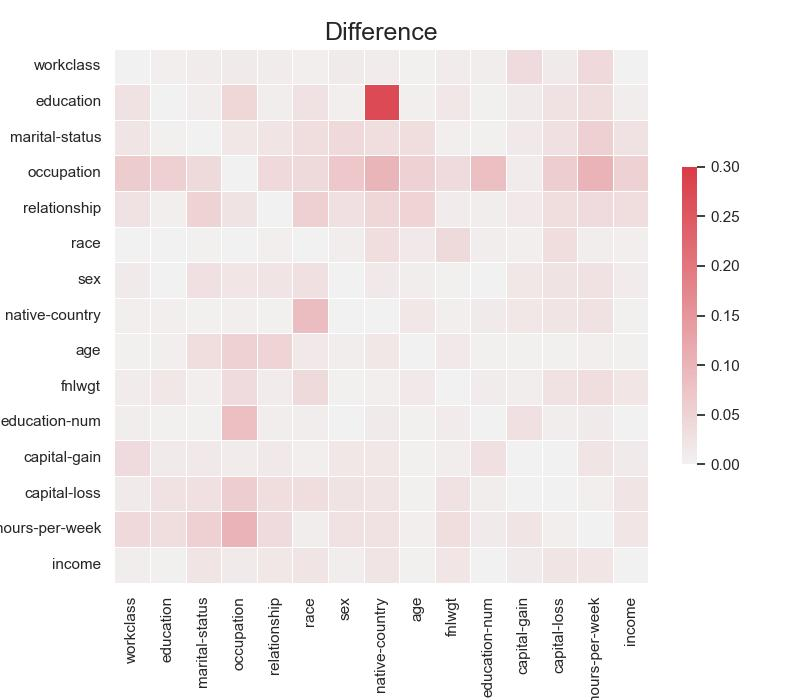
\includegraphics[width=\textwidth]{images/correlation_difference/smote.jpg}
		\caption{SMOTE}

	\end{subfigure}
	\begin{subfigure}{0.3\textwidth}
		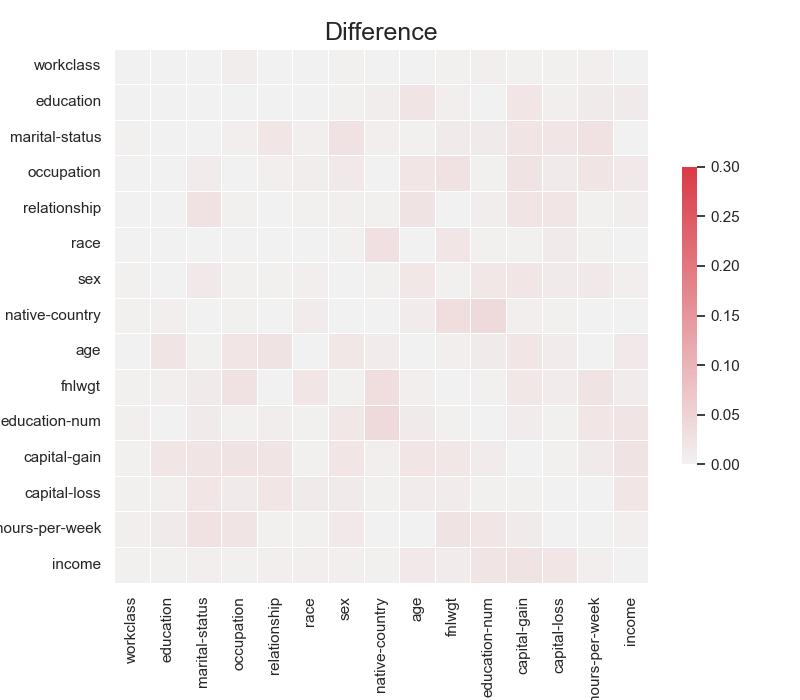
\includegraphics[width=\textwidth]{images/correlation_difference/tab-ddpm.jpg}
		\caption{TabDDPM$^{ml}_q$}
	\end{subfigure}
	\caption[Correlation plots Baseline Models]{Correlation Matrix difference for Baseline \glspl{model}.}
	\label{fig:corr_base}
\end{figure}


\begin{figure}[h]
	\begin{subfigure}{0.3\textwidth}
		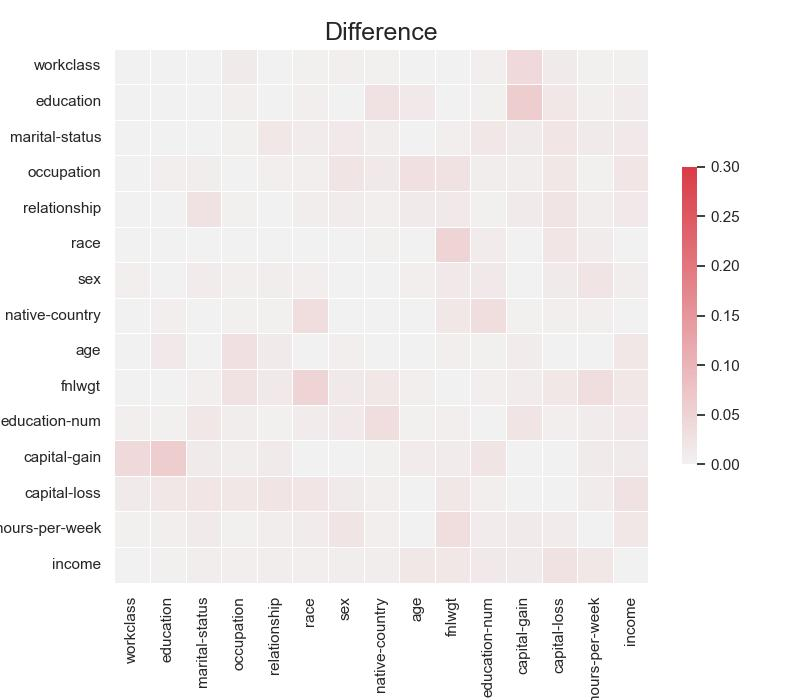
\includegraphics[width=\textwidth]{images/correlation_difference/tab-ddpm-bgm.jpg}
		\caption{TabDDPM-BGM$^{ml}_q$}
	\end{subfigure}
	\hfill
	\begin{subfigure}{0.3\textwidth}
		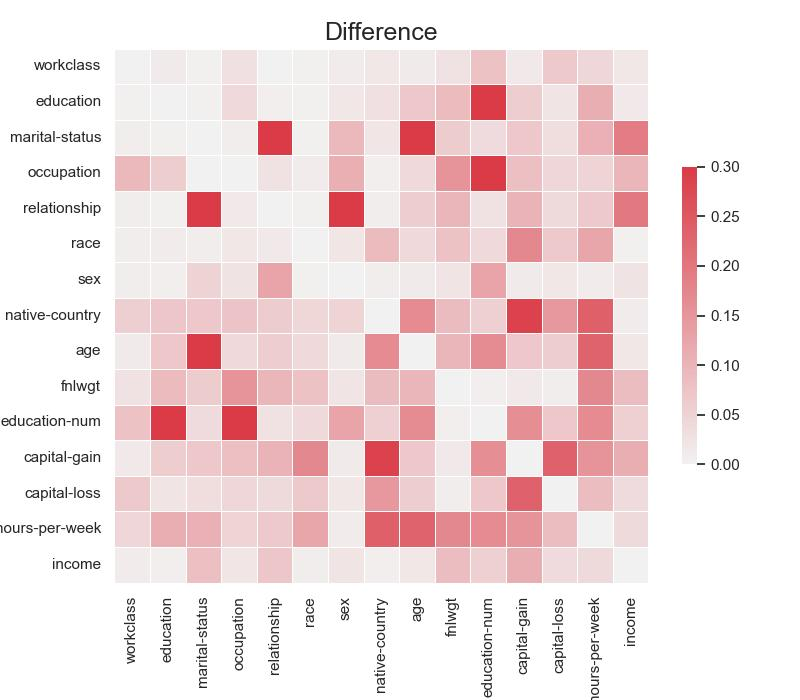
\includegraphics[width=\textwidth]{images/correlation_difference/tab-ddpm-ft.jpg}
		\caption{TabDDPM-FT$^{ml}_q$}
	\end{subfigure}
	\hfill
	\begin{subfigure}{0.3\textwidth}
		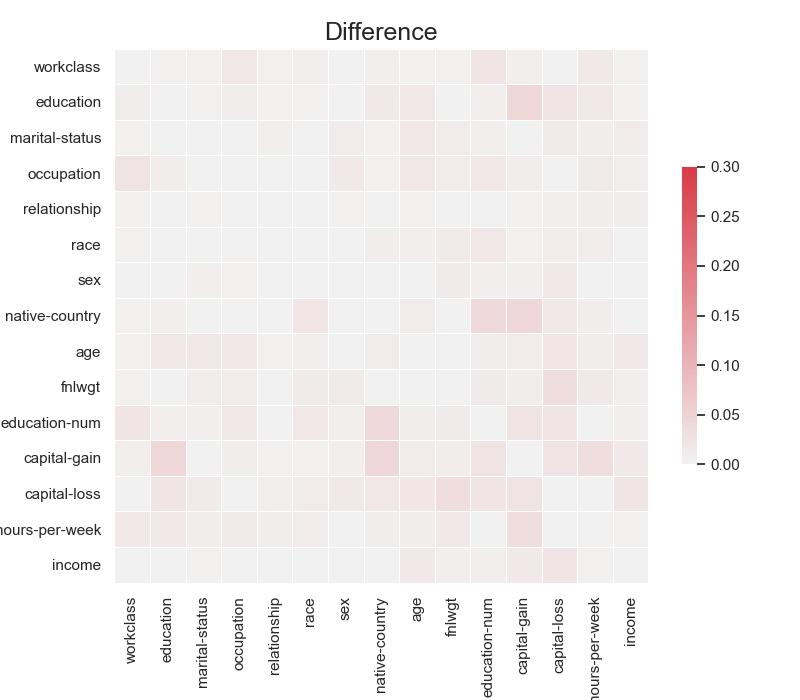
\includegraphics[width=\textwidth]{images/correlation_difference/tab-ddpm-bgm-simTune-minmax.jpg}
		\caption{TabDDPM-BGM$^{s}_m$}
	\end{subfigure}
	\caption[Correlation plots Experiment Models]{Correlation Matrix difference from selected experiment \glspl{model}.}
	\label{fig:corr_diffusion}
\end{figure}



\Autoref{fig:corr_diffusion} shows that while the TabDDPM-BGM$^{ml}$ are able to produce small correlation differences, the TabDDPM-FT$^{ml}$ is not able to reproduce
the correlation matrix of the real dataset.
The overall best correlation difference matrix is produced by TabDDPM$^{s}_m$, which is also reflected in their TabSynDex correlation score in \Autoref{tab:exp3-sim}, which is the highest across all \gls{model} versions.
Other \gls{model} version matrices do not show any noteworthy changes and are displayed in \Autoref{fig_a:corr_diff}.

\subsection{Principle Component Analysis}
\label{ch:results-pca}

A \gls{pca} is a dimensionality reduction technique that converts a dataset onto principal components \cite{brenninkmeijer2019GenerationEvaluationTabular}.
The components are then sorted according to the amount of variance from the original dataset each component is able to capture.
The following visualizations map the first two principal components, \ie the components that capture the most variance from data.


\begin{figure}[H]
	\centering
	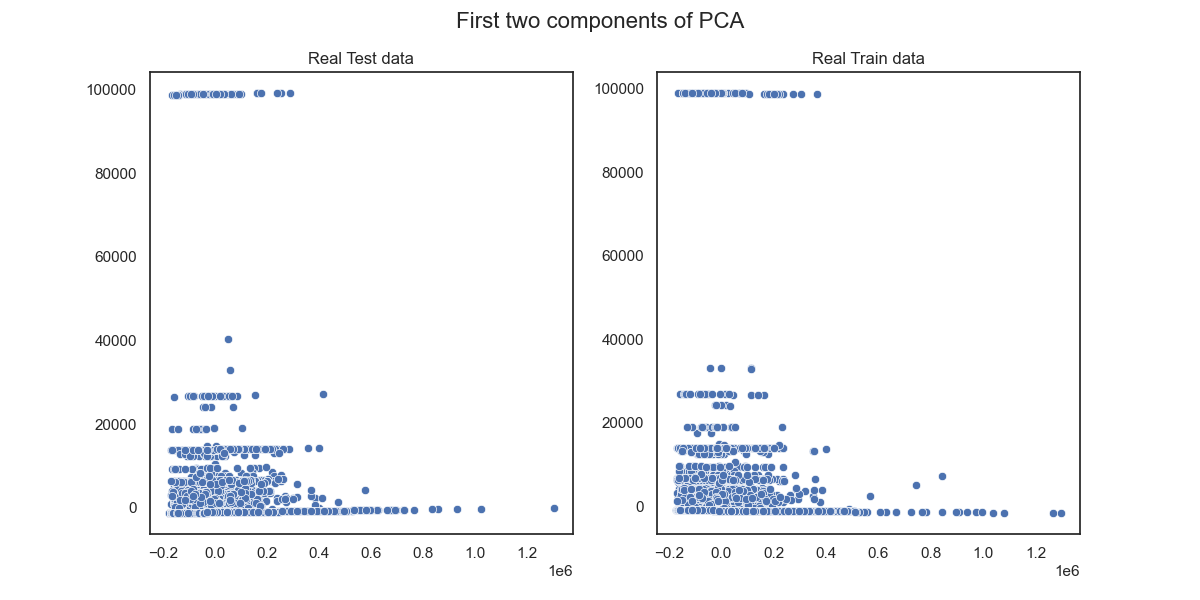
\includegraphics[width=0.7\textwidth]{images/pca/pca.png}
	\caption[PCA plot Real Data]{\gls{pca} for the real training and testing dataset}
	\label{fig:pca}
\end{figure}


\Autoref{fig:pca} shows the two \gls{pca} plots of the first two principal components from the real training and testing dataset.
One can see that the majority of values in the plots are scattered around the lower left corner (for $y<=40000$) with two accumulations of values spreading along the $x$-axis around $y=100000$ and $y=0$.
The goal of the synthetic data generation method is to produce synthetic data whose \gls{pca} plot is similar to the \gls{pca} plot of the real testing dataset.\newpage


\begin{figure}[H]
	\centering
	\begin{subfigure}{0.3\textwidth}
		\centering
		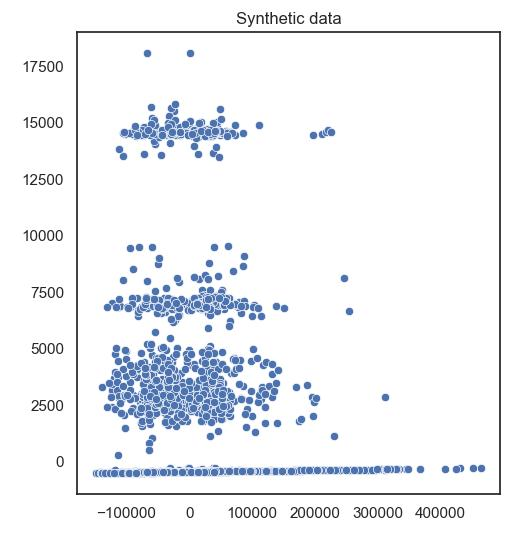
\includegraphics[width=\textwidth]{images/pca/tvae.jpg}
		\caption{TVAE$^{ml}$}
	\end{subfigure}
	\begin{subfigure}{0.3\textwidth}
		\centering
		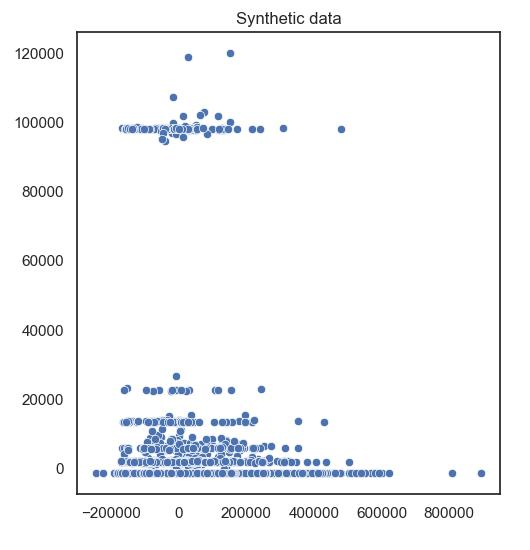
\includegraphics[width=\textwidth]{images/pca/ctabgan.jpg}
		\caption{CTABGAN$^{ml}$}
	\end{subfigure}
	\begin{subfigure}{0.3\textwidth}
		\centering
		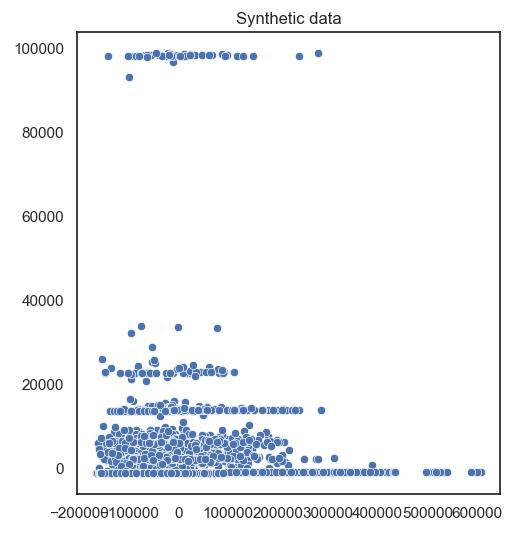
\includegraphics[width=\textwidth]{images/pca/ctabgan+.jpg}
		\caption{CTABGAN+$^{ml}$}
	\end{subfigure}
	\begin{subfigure}{0.3\textwidth}
		\centering
		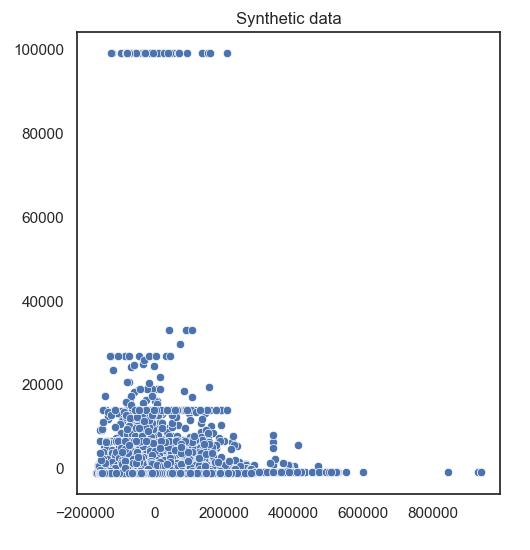
\includegraphics[width=\textwidth]{images/pca/smote.jpg}
		\caption{SMOTE}
	\end{subfigure}
	\begin{subfigure}{0.3\textwidth}
		\centering
		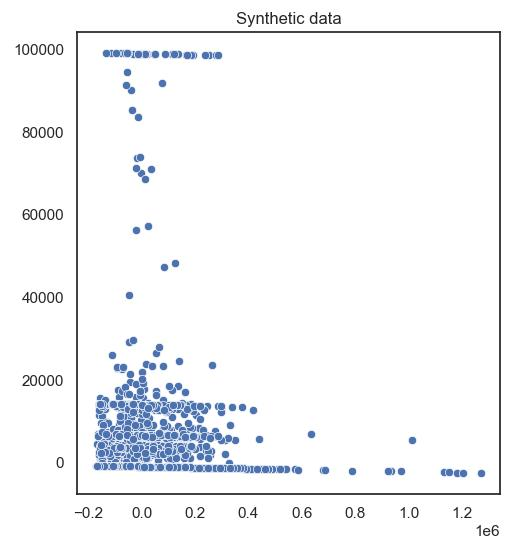
\includegraphics[width=\textwidth]{images/pca/tab-ddpm.jpg}
		\caption{TabDDPM$^{ml}_q$}
	\end{subfigure}
	\caption[PCA plots Baseline Models]{\gls{pca} for Baseline \glspl{model}.}
	\label{fig:pca_base}
\end{figure}


\begin{figure}[H]
	\centering
	\begin{subfigure}{0.3\textwidth}
		\centering
		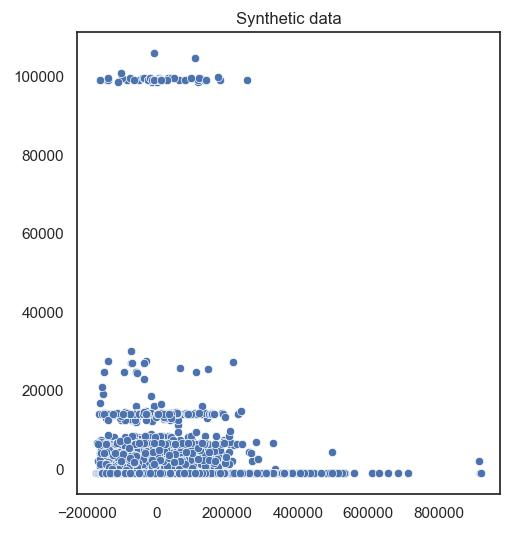
\includegraphics[width=\textwidth]{images/pca/tab-ddpm-bgm.jpg}
		\caption{TabDDPM-BGM$^{ml}_q$}
	\end{subfigure}
	\begin{subfigure}{0.3\textwidth}
		\centering
		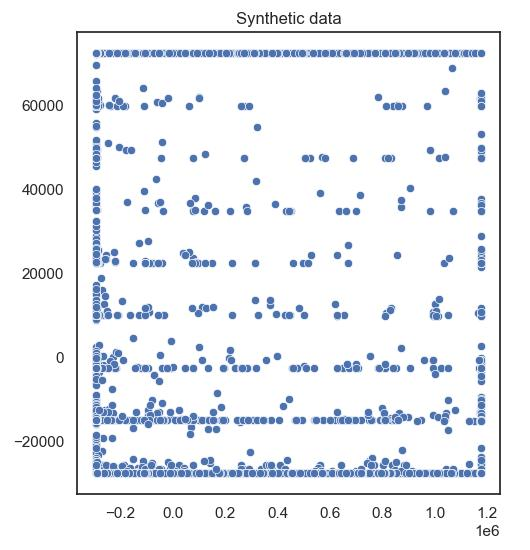
\includegraphics[width=\textwidth]{images/pca/tab-ddpm-ft.jpg}
		\caption{TabDDPM-FT$^{ml}_q$}
	\end{subfigure}


	\begin{subfigure}{0.3\textwidth}
		\centering
		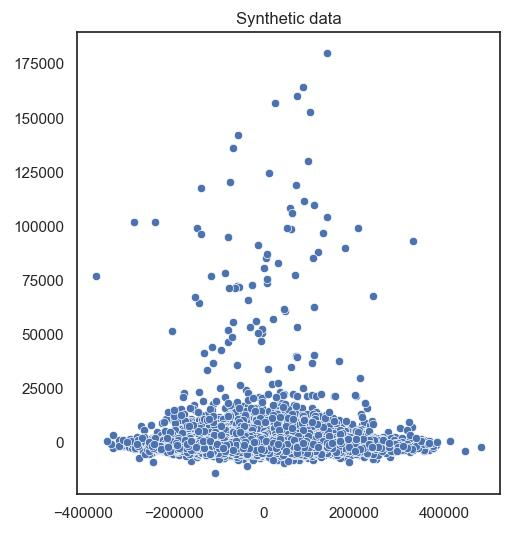
\includegraphics[width=\textwidth]{images/pca/tab-ddpm-simTune-minmax.jpg}
		\caption{TabDDPM$^{s}_m$}
	\end{subfigure}
	\begin{subfigure}{0.3\textwidth}
		\centering
		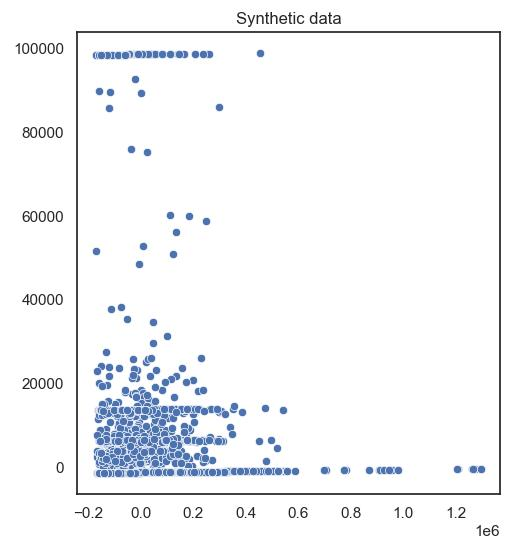
\includegraphics[width=\textwidth]{images/pca/tab-ddpm-simTune.jpg}
		\caption{TabDDPM$^{s}_q$}
	\end{subfigure}
	\caption[PCA plots Experiment Models]{\gls{pca} for selected experiment \glspl{model}.}
	\label{fig:pca_diffusion}
\end{figure}

\Autoref{fig:pca_base} shows the \gls{pca} plots for the different baseline \glspl{model}. 
All plots show some similarity with the \gls{pca}-plot from the original dataset, except for the TVAE \gls{model}. 
While it seems the CTABGAN, CTABGAN+, and TabDDPM \glspl{model} reproduce the main characteristics of the real \gls{pca} plot, they do have a few single outliers scattered.
These scatter outliers can be observed less frequently at the \gls{smote} \gls{pca} plot, which, out of the baseline \glspl{model}, recreates the original \gls{pca} plot the closest.


Out of the extended versions of TabDDPM, only the \gls{bgm} tabular processing mechanism seems to be able to produce a realistic \gls{pca}-plot (compare \Autoref{fig:pca_diffusion}).
Additionally, the min-max scaling seems to negatively affect the \gls{pca}-plot for the TabDDPM \gls{model}.
However, this did not occur for the TabDDPM-BGM \gls{model} that used min-max scaling (\Autoref{fig_a:pca_TabDDPMBM}).
This \gls{pca}-plot and the remaining \gls{model} versions plots can be found in Appendix \ref{A:pca}.

\subsection{Distribution Plot}
\label{ch:results-Distr}


For each \gls{model} version, distribution plots for each column can be found at Appendix \ref{A:distributions}, comparing the distributions of the synthetic data with the real data.
This section will highlight some interesting plots for selected \glspl{model}.

In terms of categorical distributions (\Autoref{fig:education} displays the \textit{education} column distributions as an example), all baseline \glspl{model} can reproduce the original distributions,
with CTABGAN+$^{ml}$ and TabDDPM$^{ml}_q$ replicating the original distribution best.
The \gls{bgm} tabular processing \gls{model} also reproduced the categorical distributions in a comparable way to the TabDDPM counterpart.
On the other hand, the \gls{ft} tabular processing \gls{model} could not reproduce the original distribution at all and failed to mimic the real data.

Changing the hyperparameter tuning toward the similarity score did not affect the categorical distributions in any \gls{model}.
The same is valid for changing to the min-max scaling since it only affects continuous values.
\Autoref{fig:age} shows that this observation does not extend towards continuous columns, given the column age as an example.
Across the baseline \glspl{model}, CTABGAN+$^{ml}$ and TabDDPM$^{ml}_q$ are again best able to reproduce the original data distribution of the example column.
All TabDDPM-BGM \glspl{model} produce distributions that are comparable to those produced by the baseline TabDDPM.
Again, TabDDPM-FT fails to replicate the target distributions at all.
Interestingly, the similarity score hyperparameter optimization did not affect the TabDDPM distributions to any visible extent.
However, the min-max scaling reduced the TabDDPM capability to create a realistic distribution, whose probability distributions rather follows a Gaussian distribution, failing to replicate the detailed peaks of the original dataset.
This behavior was not present in the \gls{bgm} version with min-max scaling.

Comparing all \gls{bgm} versions reveals interesting observations about the effect of applying normalizations after the tabular processing mechanisms.
Having no transformation or min-max transformation results in similar plots that can capture the overall distribution but deviate in some cases quite a lot (in the area of x=17 to 28 years).\newpage

\begin{figure}[H]
	\centering
	\begin{subfigure}{0.3\textwidth}
		\centering
		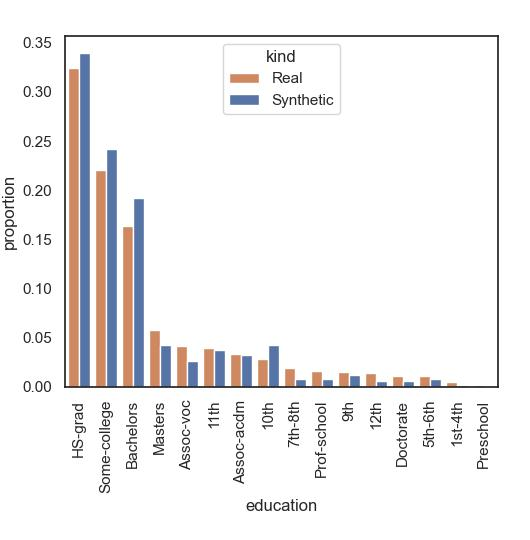
\includegraphics[width=\textwidth]{images/dist_education/tvae.jpg}
		\caption{TVAE$^{ml}$}
	\end{subfigure}
	\begin{subfigure}{0.3\textwidth}
		\centering
		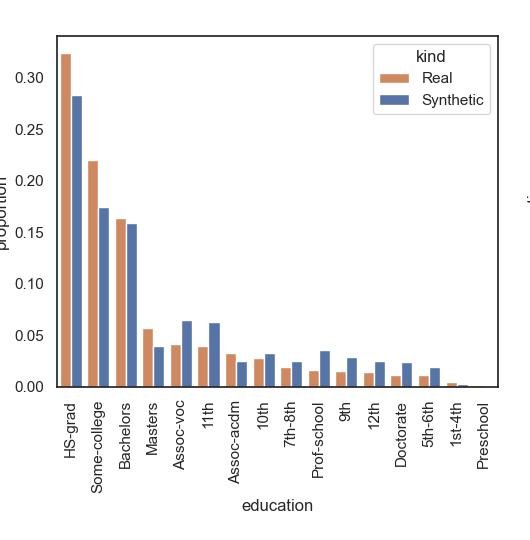
\includegraphics[width=\textwidth]{images/dist_education/ctabgan.jpg}
		\caption{CTABGAN$^{ml}$}
	\end{subfigure}
	\begin{subfigure}{0.3\textwidth}
		\centering
		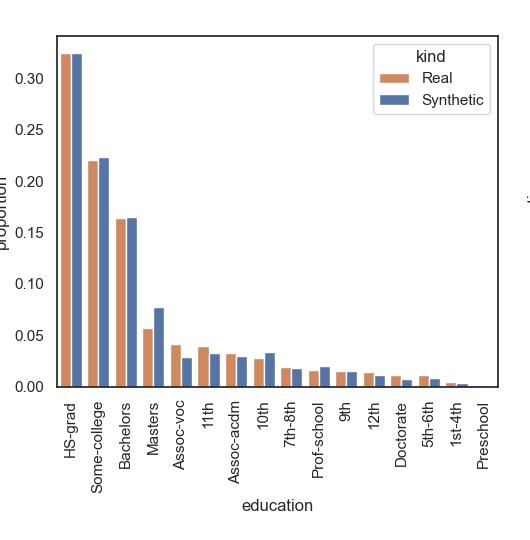
\includegraphics[width=\textwidth]{images/dist_education/ctabgan+.jpg}
		\caption{CTABGAN+$^{ml}$}
	\end{subfigure}


	\begin{subfigure}{0.3\textwidth}
		\centering
		\includegraphics[width=\textwidth]{images/dist_education/SMOTE.jpg}
		\caption{SMOTE}
	\end{subfigure}
	\begin{subfigure}{0.3\textwidth}
		\centering
		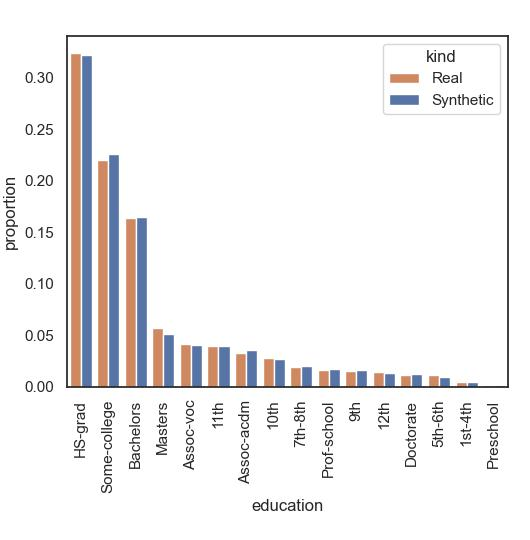
\includegraphics[width=\textwidth]{images/dist_education/tab-ddpm.jpg}
		\caption{TabDDPM$^{ml}_q$}
	\end{subfigure}  


	\begin{subfigure}{0.3\textwidth}
		\centering
		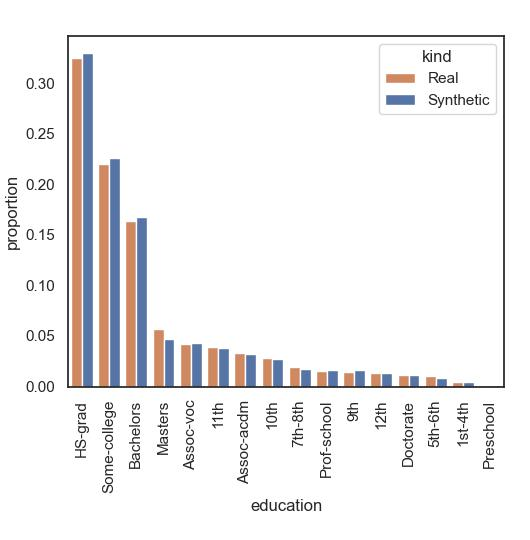
\includegraphics[width=\textwidth]{images/dist_education/tab-ddpm-bgm.jpg}
		\caption{TabDDPM-BGM$^{ml}_q$}
	\end{subfigure}
	\begin{subfigure}{0.3\textwidth}
		\centering
		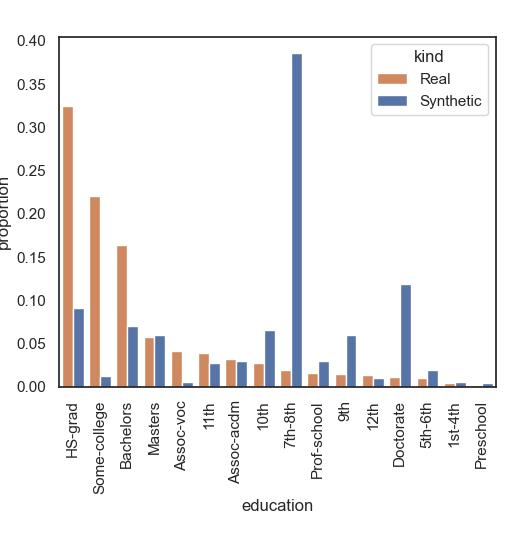
\includegraphics[width=\textwidth]{images/dist_education/tab-ddpm-ft.jpg}
		\caption{TabDDPM-FT$^{ml}_q$}
	\end{subfigure}
	\caption[Distribution Plots Categorical]{\textit{Education} column for baseline \glspl{model}.}
	\label{fig:education}
\end{figure}

Quantile transformation (TabDDPM-BGM$^{s}_q$) reduces the difference in this area, but an oversampling of entries with an age of 90 occurred.
Interestingly, out of all \gls{bgm} variations, the \gls{model} tuned after the machine learning efficacy (TabDDPM-BGM$^{ml}_q$) was best able to capture the distribution.
Looking at its \textit{age} distribution plot, it can be observed that big differences from the real data are few.
Nevertheless, undersampling of certain ages is present in the synthetic data.
However, one can observe that this is usually compensated with an oversampling of an age value close to it
(\eg undersampling of age x=17-18 is compensated by an oversampling of age x=19-20).\newpage


\begin{figure}[H]
	\centering
	\begin{subfigure}{0.3\textwidth}
		\centering
		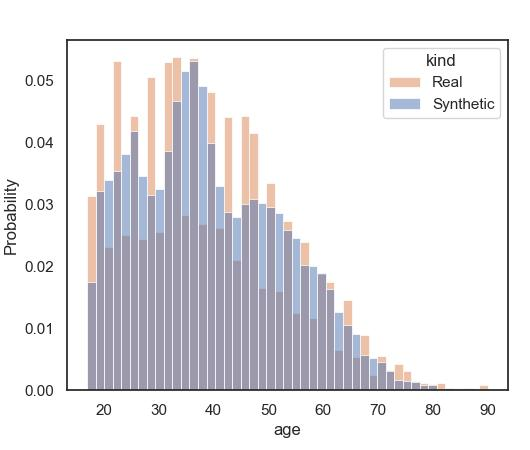
\includegraphics[width=\textwidth]{images/dist_age/tvae.jpg}
		\caption{TVAE$^{ml}$}
	\end{subfigure}
	\begin{subfigure}{0.3\textwidth}
		\centering
		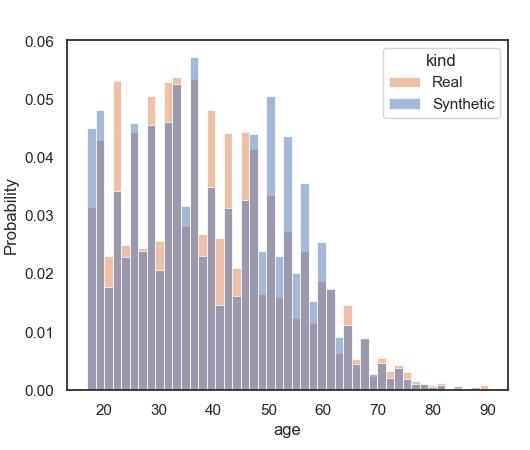
\includegraphics[width=\textwidth]{images/dist_age/ctabgan.jpg}
		\caption{CTABGAN$^{ml}$}
	\end{subfigure}
	\begin{subfigure}{0.3\textwidth}
		\centering
		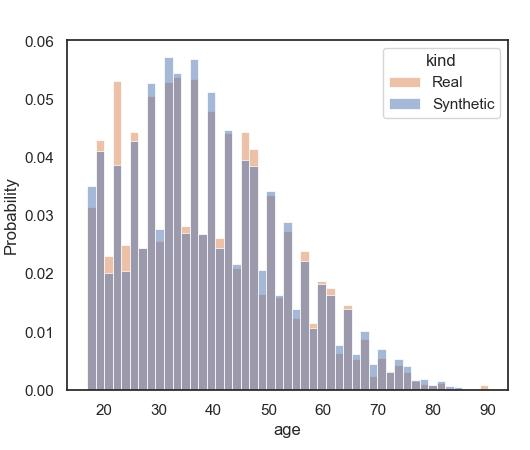
\includegraphics[width=\textwidth]{images/dist_age/ctabgan+.jpg}
		\caption{CTABGAN+$^{ml}$}
	\end{subfigure}


	\begin{subfigure}{0.3\textwidth}
		\centering
		\includegraphics[width=\textwidth]{images/dist_age/SMOTE.jpg}
		\caption{SMOTE}
	\end{subfigure}
	\begin{subfigure}{0.3\textwidth}
		\centering
		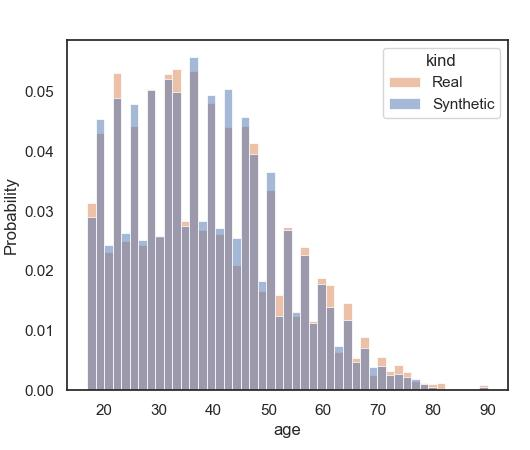
\includegraphics[width=\textwidth]{images/dist_age/tab-ddpm.jpg}
		\caption{TabDDPM$^{ml}_q$}
	\end{subfigure}
	\begin{subfigure}{0.3\textwidth}
		\centering
		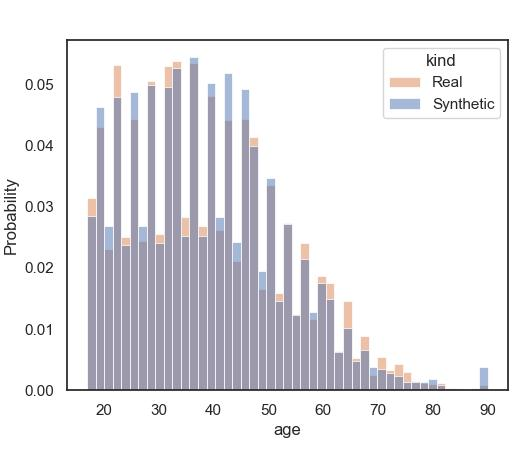
\includegraphics[width=\textwidth]{images/dist_age/tab-ddpm-simTune.jpg}
		\caption{TabDDPM$^{s}_q$}
	\end{subfigure}


	\begin{subfigure}{0.3\textwidth}
		\centering
		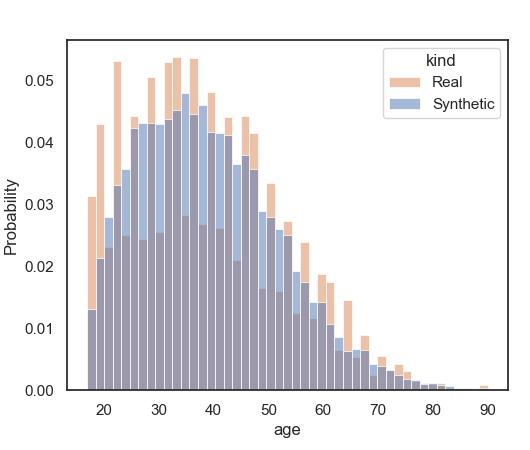
\includegraphics[width=\textwidth]{images/dist_age/tab-ddpm-simTune-minmax.jpg}
		\caption{TabDDPM$^{s}_m$}
	\end{subfigure}
	\begin{subfigure}{0.3\textwidth}
		\centering
		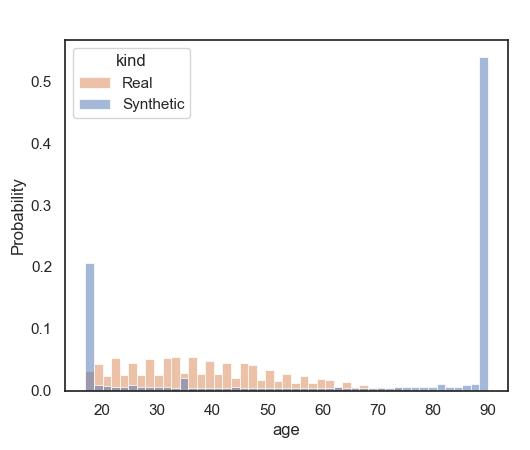
\includegraphics[width=\textwidth]{images/dist_age/tab-ddpm-ft.jpg}
		\caption{TabDDPM-FT$^{ml}_q$}
	\end{subfigure}
	\begin{subfigure}{0.3\textwidth}
		\centering
		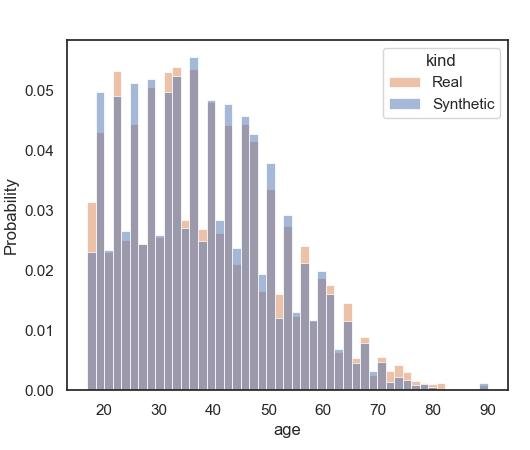
\includegraphics[width=\textwidth]{images/dist_age/tab-ddpm-bgm.jpg}
		\caption{TabDDPM-BGM$^{ml}_q$}
	\end{subfigure}


	\begin{subfigure}{0.3\textwidth}
		\centering
		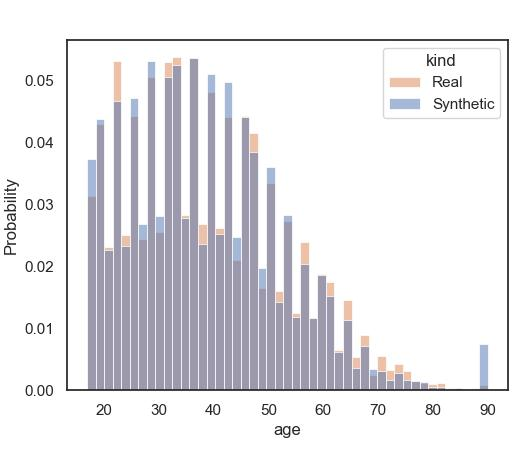
\includegraphics[width=\textwidth]{images/dist_age/tab-ddpm-bgm-simTune.jpg}
		\caption{TabDDPM-BGM$^{s}_q$}
	\end{subfigure}
	\begin{subfigure}{0.3\textwidth}
		\centering
		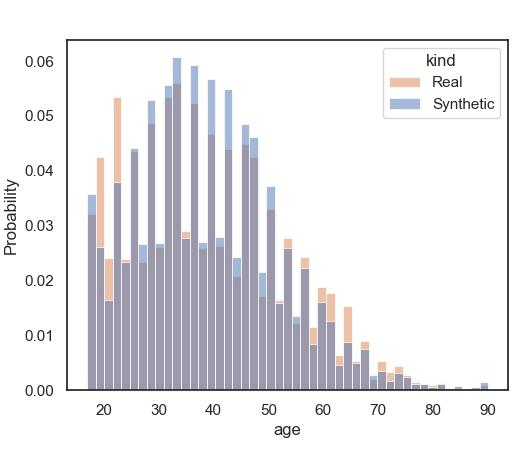
\includegraphics[width=\textwidth]{images/dist_age/tab-ddpm-bgm-simTune-minmax.jpg}
		\caption{TabDDPM-BGM$^{s}_m$}
	\end{subfigure}
	\begin{subfigure}{0.3\textwidth}
		\centering
		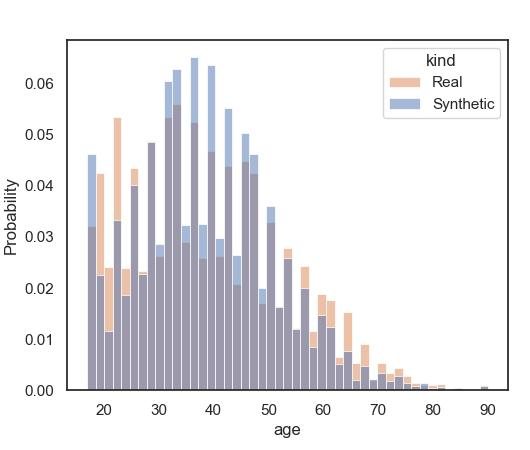
\includegraphics[width=\textwidth]{images/dist_age/tab-ddpm-bgm-simTune-none.jpg}
		\caption{TabDDPM-BGM$^{s}_n$}
	\end{subfigure}
	\caption[Distribution Plots Continuous]{\textit{Age} column for selected \gls{model} versions. Please note that the Y-axis range may vary due to the range of the synthetic data.}
	\label{fig:age}
\end{figure}
\newpage


\subsection{Cumulative Distribution Function}

\begin{figure}[H]
	\centering
	\begin{subfigure}{0.3\textwidth}
		\centering
		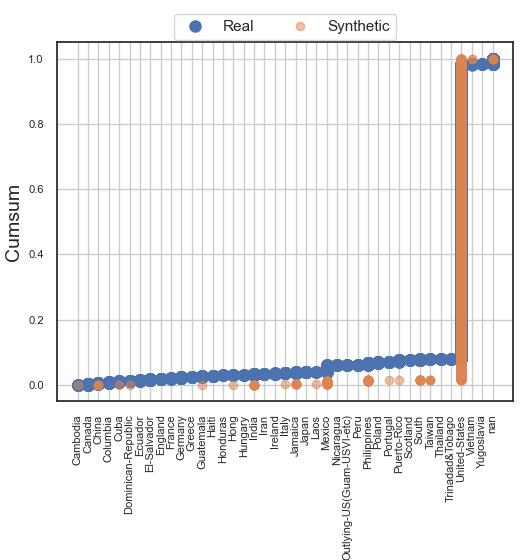
\includegraphics[width=\textwidth]{images/cdf/tvae.jpg}
		\caption{TVAE$^{ml}$}
	\end{subfigure}
	\begin{subfigure}{0.3\textwidth}
		\centering
		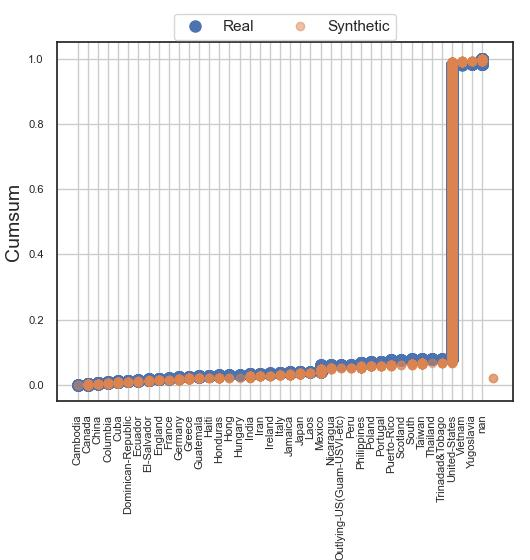
\includegraphics[width=\textwidth]{images/cdf/ctabgan+.jpg}
		\caption{CTABGAN+$^{ml}$}
	\end{subfigure}
	\begin{subfigure}{0.3\textwidth}
		\centering
		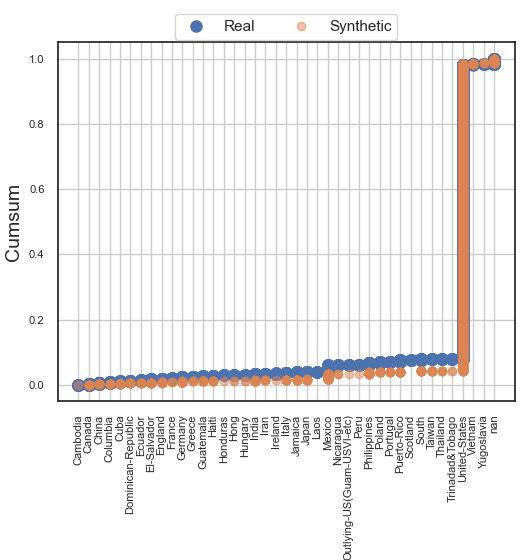
\includegraphics[width=\textwidth]{images/cdf/tab-ddpm-bgm.jpg}
		\caption{TabDDPM-BGM$^{ml}_q$}
	\end{subfigure}


	\begin{subfigure}{0.3\textwidth}
		\centering
		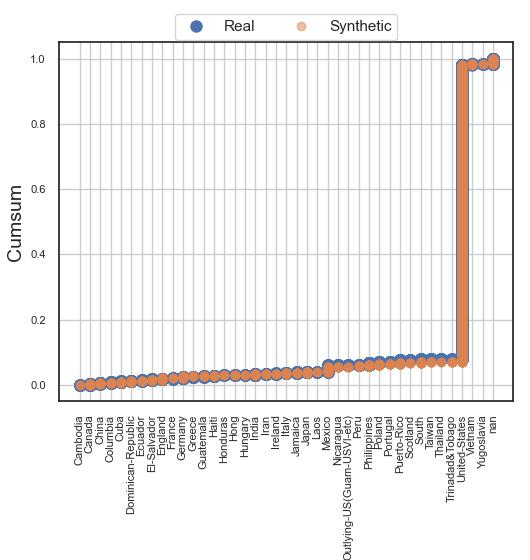
\includegraphics[width=\textwidth]{images/cdf/tab-ddpm-bgm-simTune.jpg}
		\caption{TabDDPM-BGM$^{s}_q$}
	\end{subfigure}
	\begin{subfigure}{0.3\textwidth}
		\centering
		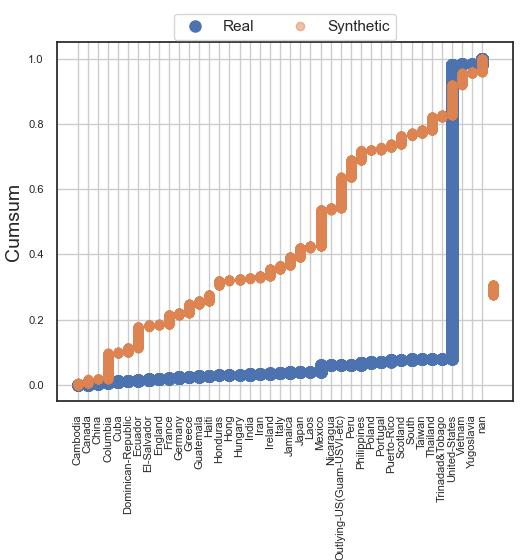
\includegraphics[width=\textwidth]{images/cdf/tab-ddpm-ft.jpg}
		\caption{TabDDPM-FT$^{ml}_q$}
	\end{subfigure}
	\begin{subfigure}{0.3\textwidth}
		\centering
		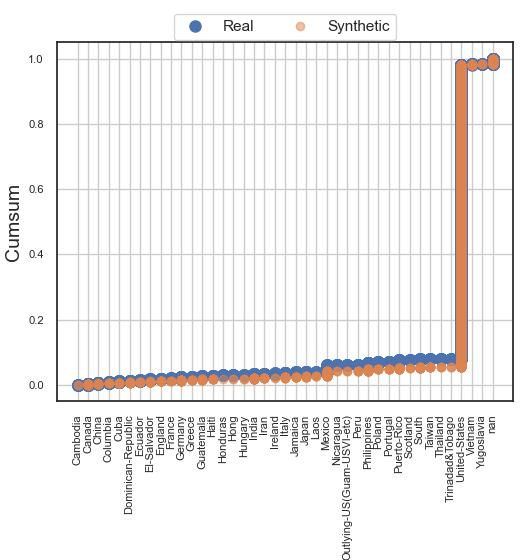
\includegraphics[width=\textwidth]{images/cdf/tab-ddpm.jpg}
		\caption{TabDDPM$^{ml}_q$}
	\end{subfigure}


	\begin{subfigure}{0.3\textwidth}
		\centering
		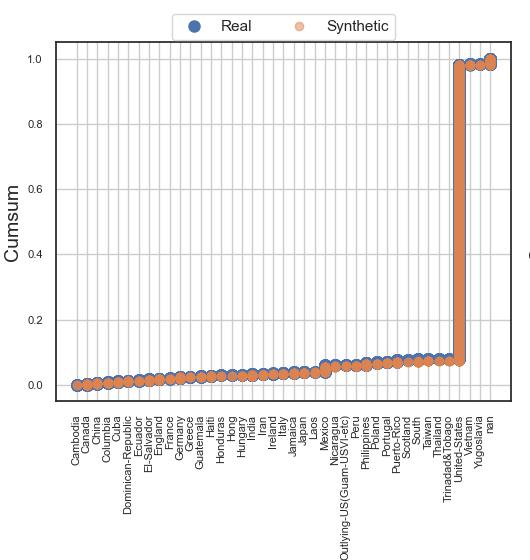
\includegraphics[width=\textwidth]{images/cdf/tab-ddpm-simTune-minmax.jpg}
		\caption{TabDDPM$^{s}_m$}
	\end{subfigure}
	\begin{subfigure}{0.3\textwidth}
		\centering
		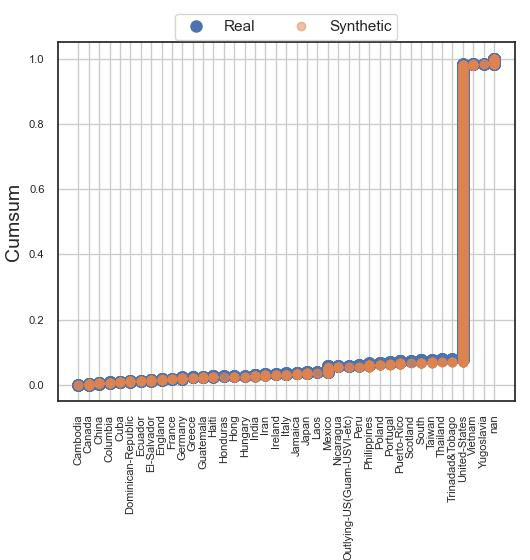
\includegraphics[width=\textwidth]{images/cdf/tab-ddpm-bgm-simTune-minmax.jpg}
		\caption{TabDDPM-BGM$^{s}_m$}
	\end{subfigure}
	\caption[CDF native-country]{\gls{cdf} plots for selected model versions for categorical the column "native-country" of the adult income dataset \cite{Dua:2019}}
	\label{fig:cdf}
\end{figure}

All \gls{cdf} plots can be found in Appendix \ref{A:cumsum}.
The plots show that the \glspl{cdf} of the synthetic data created by CTABGAN+$^{ml}$ and TabDDPM$^{ml}_q$ come closest to
the \glspl{cdf} of the real data across the baseline \glspl{model} (best visible for columns \textit{native-country} or \textit{hours-per-week}, compare \Autoref{fig:cdf, fig:cdf_hpw}).
The selected plots in \Autoref{fig:cdf, fig:cdf_hpw} show how the \gls{ft} tabular processing failed again to reproduce the original datas \gls{cdf}.
TabDDPM-BGM, on the other hand, produced synthetic data, whose \gls{cdf} correctly mimics the \gls{cdf} of the real data.
One could argue that TabDDPM and TabDDPM-BGM that have been tuned after the similarity score are slightly better able to
reproduce \gls{cdf} plots for categorical columns whose categories are imbalanced (\eg see column \textit{native-country}, where the majority of values equal \textit{United-States}).
This improvement is more prominent for the \gls{bgm} version.
The min-max scaling greatly affected the TabDDPM version and "smoothed out" its \glspl{cdf}.
This phenomenon was not present in the TabDDPM-BGM version with min-max scaling.

\begin{figure}[H]
	\centering
	\begin{subfigure}{0.3\textwidth}
		\centering
		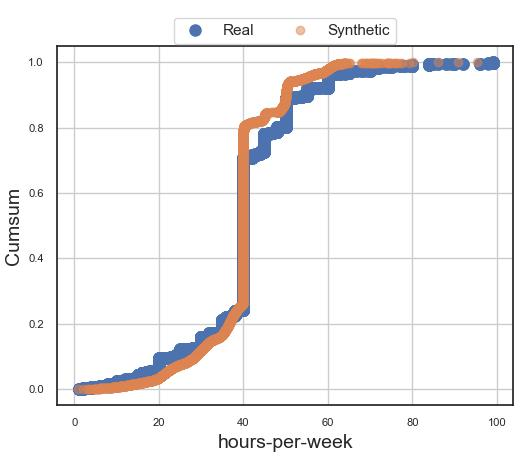
\includegraphics[width=\textwidth]{images/cdf_hpw/tvae.jpg}
		\caption{TVAE$^{ml}$}
	\end{subfigure}
	\begin{subfigure}{0.3\textwidth}
		\centering
		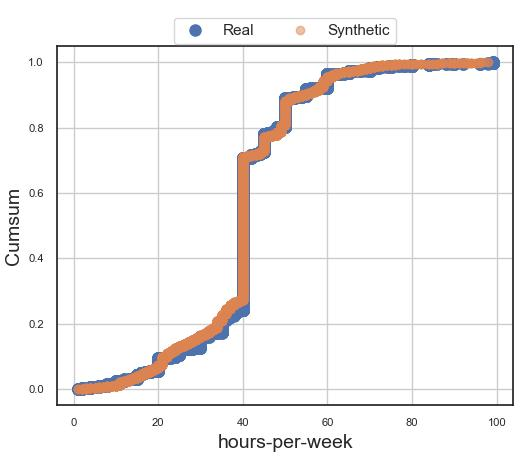
\includegraphics[width=\textwidth]{images/cdf_hpw/ctabgan+.jpg}
		\caption{CTABGAN+$^{ml}$}
	\end{subfigure}
	\begin{subfigure}{0.3\textwidth}
		\centering
		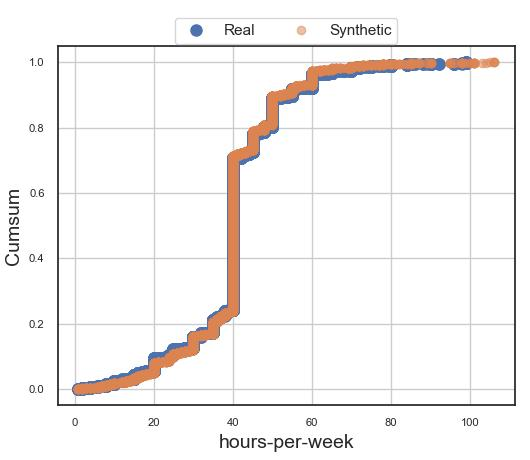
\includegraphics[width=\textwidth]{images/cdf_hpw/tab-ddpm-bgm.jpg}
		\caption{TabDDPM-BGM$^{ml}_q$}
	\end{subfigure}


	\begin{subfigure}{0.3\textwidth}
		\centering
		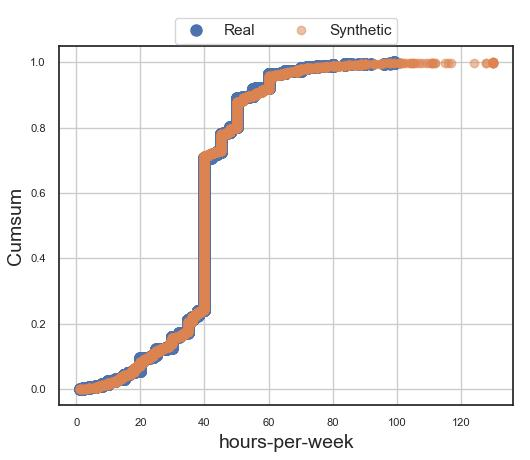
\includegraphics[width=\textwidth]{images/cdf_hpw/tab-ddpm-bgm-simTune.jpg}
		\caption{TabDDPM-BGM$^{s}_q$}
	\end{subfigure}
	\begin{subfigure}{0.3\textwidth}
		\centering
		\includegraphics[width=\textwidth]{images/cdf_hpw/tab-ddpm-ft.jpg}
		\caption{TabDDPM-FT$^{ml}_q$}
	\end{subfigure}
	\begin{subfigure}{0.3\textwidth}
		\centering
		\includegraphics[width=\textwidth]{images/cdf_hpw/tab-ddpm.jpg}
		\caption{TabDDPM$^{ml}_q$}
	\end{subfigure}


	\begin{subfigure}{0.3\textwidth}
		\centering
		\includegraphics[width=\textwidth]{images/cdf_hpw/tab-ddpm-simTune-minmax.jpg}
		\caption{TabDDPM$^{s}_m$}
	\end{subfigure}
	\begin{subfigure}{0.3\textwidth}
		\centering
		\includegraphics[width=\textwidth]{images/cdf_hpw/tab-ddpm-bgm-simTune-minmax.jpg}
		\caption{TabDDPM-BGM$^{s}_m$}
	\end{subfigure}
	\caption[CDF hours-per-week]{\gls{cdf} plots for selected model versions for the numerical column "hours-per-week" of the adult income dataset \cite{Dua:2019}}
	\label{fig:cdf_hpw}
\end{figure}



\newpage
\section{Discussion}
\label{ch:results-discussion}
The goal of this thesis was to investigate the performance of adding the tabular processing mechanisms to the TabDDPM \gls{model} (\gls{rq}1) and
to expand upon the already existing machine learning efficacy evaluation performed by \cite{kotelnikov2022TabDDPMModellingTabular} through the TabSynDex similarity score metrics proposed by \cite{chundawat2022UniversalMetricRobust}.

\subsection*{Analysis of Visual and Numerical Results}

\begin{table}[h]
	\centering
	\begin{tabular}{lrrr}
		\toprule
		\textbf{Model}        & \textbf{Accuracy} & \textbf{F1}    & \textbf{ROC-AUC} \\
		\midrule
		Real                  & 0.874              & 0.815          & 0.928            \\
		TVAE$^{ml}$           & 0.845              & 0.780          & 0.900            \\
		SMOTE                 & 0.858              & 0.791          & 0.910            \\
		CTABGAN$^{ml}$        & 0.850              & 0.775          & 0.900            \\
		CTABGAN+$^{ml}$       & 0.855              & 0.775          & 0.907            \\
		TabDDPM$^{ml}_q$      & 0.860              & 0.794          & 0.913            \\
		TabDDPM-BGM$^{ml}_q$  & \textbf{0.863}     & \textbf{0.798} & \textbf{0.916}   \\
		TabDDPM-FT$^{ml}_q$   & 0.785              & 0.552          & 0.821            \\
		CTABGAN$^{s}_q$       & 0.850              & 0.776          & 0.900            \\
		CTABGAN+$^{s}$        & 0.851              & 0.768          & 0.902            \\
		TVAE$^{s}$            & 0.845              & 0.780          & 0.900            \\
		TabDDPM$^{s}_q$       & 0.856              & 0.782          & 0.908            \\
		TabDDPM-BGM$^{s}_q$   & 0.859              & 0.792          & 0.911            \\
		TabDDPM-FT$^{s}_q$    & 0.766              & 0.451          & 0.712            \\
		TabDDPM$^{s}_m$       & 0.856              & 0.778          & 0.910            \\
		TabDDPM-BGM$^{s}_m$   & 0.857              & 0.787          & 0.909            \\
		TabDDPM-BGM$^{s}_{n}$ & 0.855              & 0.784          & 0.907            \\
		\bottomrule
		\multicolumn{4}{c}{}\\[-0.6em]
	\end{tabular}
	\caption[Overview all ML efficacy results]{Overview of all CatBoost machine learning efficacy results for all tested model versions.}
	\label{tab:ml-all}
\end{table}


\begin{table}[h]
	\centering
	\begin{tabular}{lrrrrrr}
		\toprule
		\textbf{Model}        & \textbf{Similarity Score} & \textbf{Basic} & \textbf{Correlation} & \textbf{ML}    & \textbf{Support} & \textbf{pMSE}  \\
		\midrule
		Real                  & 0.960                     & 0.992          & 0.943                & 0.998          & 0.984            & 0.882          \\
		TVAE$^{ml}$           & 0.658                     & 0.854          & 0.814                & 0.962          & 0.657            & 0.000          \\
		SMOTE                 & 0.723                     & 0.953          & 0.865                & 0.992          & 0.804            & 0.000          \\
		CTABGAN$^{ml}$        & 0.741                     & 0.940          & 0.832                & 0.984          & 0.947            & 0.000          \\
		CTABGAN+$^{ml}$       & 0.750                     & 0.969          & 0.882                & 0.990          & 0.892            & 0.019          \\
		TabDDPM$^{ml}_q$      & 0.759                     & 0.973          & 0.919                & 0.992          & 0.874            & 0.035          \\
		TabDDPM-BGM$^{ml}_q$  & 0.742                     & 0.964          & 0.918                & \textbf{0.996} & 0.831            & 0.000          \\
		TabDDPM-FT$^{ml}_q$   & 0.595                     & 0.495          & 0.648                & 0.869          & 0.963            & 0.000          \\
		CTABGAN$^{s}$         & 0.740                     & 0.938          & 0.833                & 0.984          & 0.947            & 0.000          \\
		CTABGAN+$^{s}$        & 0.784                     & 0.970          & 0.888                & 0.987          & 0.908            & 0.167          \\
		TVAE$^{s}$            & 0.658                     & 0.856          & 0.815                & 0.962          & 0.656            & 0.000          \\
		TabDDPM$^{s}_q$       & 0.852                     & 0.976          & 0.921                & 0.991          & 0.952            & 0.420          \\
		TabDDPM-BGM$^{s}_q$   & 0.857                     & \textbf{0.982} & 0.858                & 0.991          & 0.920            & 0.532          \\
		TabDDPM-FT$^{s}_q$    & 0.588                     & 0.512          & 0.619                & 0.818          & \textbf{0.992}   & 0.000          \\
		TabDDPM$^{s}_m$       & \textbf{0.869}            & 0.938          & \textbf{0.930}       & 0.990          & 0.928            & \textbf{0.558} \\
		TabDDPM-BGM$^{s}_m$   & 0.856                     & 0.981          & 0.913                & 0.992          & 0.915            & 0.476          \\
		TabDDPM-BGM$^{s}_{n}$ & 0.833                     & 0.975          & 0.916                & 0.992          & 0.915            & 0.369          \\
		\bottomrule
		\multicolumn{7}{c}{}\\[-0.6em]
	\end{tabular}
	\caption[Overview all TabSynDex results]{Overview of all TabSynDex score results for all tested model versions.}
	\label{tab:sim-all}
\end{table}


Based on the obtained results, it is evident that the processing mechanism for \gls{ft} has failed and is not advisable.
Despite having the highest overall support score, all other measurements and visual representations indicate that the \gls{model} could not generate synthetic data that closely resembles the original dataset.
The reason why the \gls{ft} processing does not work well even though it performed well in the cell imputation task \cite{zheng2022DiffusionModelsMissing} remains unclear.
As a consequence, the TabDDPM-FT variations will not be further discussed or analyzed.

The \gls{bgm} processor variant was able to produce not only good numerical but also visual results.
In terms of machine learning efficacy, the TabDDPM-BGM$^{ml}_q$ version shows the best machine learning efficacy performance across all tested metrics (\Autoref{tab:ml-all}: Accuracy, F1 and AUC-ROC and \Autoref{tab:sim-all}: ML).
However, the advantage over its simpler counterpart TabDDPM$^{ml}_q$ is only marginal (+0.003\%-points).
Overall, \glspl{model} with hyperparameters tuned towards machine learning efficacy outperform \glspl{model} with hyperparameters tuned towards similarity score in the machine learning efficacy scores, as one would expect.
The results of the non-diffusion baseline \glspl{model} show that the \gls{smote} approach is a reliable sampling technique when the synthetic data will be used in a machine-learning scenario.
Its machine learning efficacy results are superior to the other non-diffusion baseline \glspl{model}, while the \gls{model} is overall less complex.
For other scenarios, CTABGAN+ achieves the best overall performance in terms of numerical and visual results for non-diffusion-based \glspl{model}.
Nevertheless, the best-found CTABGAN+ version is inferior to the best-found diffusion \gls{model}.

Changing the tuning strategy to the similarity score allowed several observations to be made.
Firstly for the non-diffusion \glspl{model}', metric results had not significantly changed after switching to similarity score tuning.
All of their metric scores stayed roughly the same, with the exception of CTABGAN+.
Only for this \gls{model}, a similarity tuning resulted in a noteworthy metric increase, especially for its \gls{pmse} score, which increased by +0.14\%-points.

Diffusion \glspl{model}, on the other hand, showed more noteworthy changes in their numerical metric results.
Overall, diffusion \glspl{model} with a similarity score tuning show reduced machine learning efficacy metric scores compared to their machine learning efficacy counterparts.
While this reduction is relatively small, the similarity metrics have increased significantly.
Specifically, through the adjustment of the hyperparameters towards the similarity score, which includes the \gls{pmse} score, an increase in the \gls{pmse} score was notably achieved.
Especially for diffusion \glspl{model}, this big increase in the \gls{pmse} score is worth highlighting.
For \glspl{model} such as TabDDPM and TabDDPM-BGM, this similarity tuning resulted in \gls{pmse} values increasing to a score between $0.42$ and $0.55$.
The same tuning strategy did not affect the \gls{pmse} score of baseline \glspl{model} like TVAE or CTABGAN; only CTABGAN+ was affected but at a lower amplitude compared to diffusion \glspl{model}.
These \gls{pmse} scores indicate, that almost all non-diffusion baseline \glspl{model} failed to produce data that is non-differentiable from the real data by a logistic regression \gls{model}.
This finding aligns with the observation made by \textcite{chundawat2022UniversalMetricRobust}, who also observe that all of their tested \glspl{model} (mainly \gls{gan}-based) achieve a \gls{pmse} of 0.
The experiments of \textcite{chundawat2022UniversalMetricRobust} only identified one \gls{model}, a \gls{gan} \gls{model} with gradient penalty and Wasserstein distance, which was able to achieve a peak \gls{pmse} score of $0.4$ (scores are not comparable, since a different dataset was used).
Overall, this indicates that diffusion-based \glspl{model} are better able to produce synthetic data that is harder to differentiate from its real counterpart.

In addition to the increase of the \gls{pmse} score, the other metrics that make up the similarity score have also increased, but on a smaller scale.
Only correlation values got decreased slightly through the similarity tuning.
This observation holds for TabDDPM and TabDDPM-BGM but not for the baseline \glspl{model} (TVAE and CTABGAN), whose metric results remained unchanged after switching the tuning strategy.
This indicates that the importance of hyperparameter tuning is much higher for diffusion \glspl{model} in tabular data synthesis, as their tuning strategy affects the metric outcomes significantly.

Replacing the quantile transform function with min-max scaling for the TabDDPM (TabDDPM$^{s}_m$) has led to the highest overall similarity score.
It scored highest in both correlation and \gls{pmse}, leading to a high overall similarity score.
According to \cite{scikit-learndevelopers2023QuantileTransformer}, the quantile transform function is a non-linear transformation that may distort correlations between variables.
This is also observable in the correlation metric score, where TabDDPM$^{s}_q$ and TabDDPM-BGM$^{s}_q$ have a lower correlation score than their min-max scaling counterpart.
However, it is essential to also take into consideration the visual results.
Although the correlation difference plot of TabDDPM$^{s}_m$ appears satisfactory, the distribution and \gls{cdf} plot of continuous columns (compare \Autoref{fig_a:dist_3_c,fig_a:cumsum_3_c}) look worse when compared to those of other \glspl{model}.
The continuous plots of TabDDPM$^{s}_m$ lack details and rather approximate the original distribution.
The \gls{model}'s quantile transform counterpart TabDDPM$^{s}_q$ does not show this behavior, producing overall more realistic plots.
This indicates that the min-max scaling, which is applied to the numerical columns, causes this kind of behavior.
Since min-max scaling scales the data according to the minimum and maximum value with the column, it is susceptible to outliers.
This results in a bad normalization if even one value in the column is unusually large or small.
The \gls{bgm} processor also makes use of a form of min-max encoding in their "general transform" \cite[p. 7]{zhao2022CTABGANEnhancingTabular} (compare \Autoref{ch:BGMProcessor}).
However, \textcite{zhao2022CTABGANEnhancingTabular} emphasizes as well that this encoding should only be applied to simple continuous distributions like a single-mode Gaussian distribution.
TabDDPM-BGM$^{s}_m$ does not show this behavior even though min-max scaling is applied.
A possible explanation for why the TabDDPM-BGM variants are not affected by a min-max scaling in the same way as TabDDPM is related to the mode-specific normalization.
Recall that mode-specific normalization transforms numerical columns into a vector consisting of an $\alpha$ and a $\beta$ part.
The $\alpha$ part is the normalized value according to the most likely mode, which is indicated in the \gls{oh} vector $\beta$.
The \textit{TabularProcessor} splits the $\alpha$ and $\beta$ parts up and assigns them to the numerical and categorical output arrays respectively.
This was required since the diffusion for numerical and categorical values is different (Gaussian diffusion for numerical and Multinomial diffusion for categorical).
Only after this, the normalization through min-max is applied (and only to the numerical values). 
But since all the $\alpha$ values are already normalized, the impact of an additional normalization through the min-max function is most likely reduced.

In summary, the following observations could be made:

\begin{itemize}
	\item The processing mechanism for \gls{ft} has failed and is not advisable, as it could not generate synthetic data that closely resembles the original dataset.
	\item The \gls{bgm} processor produced good numerical and visual results.
	\item TabDDPM-BGM$^{ml}_q$ shows the best machine learning efficacy performance across all tested \glspl{model}.
	\item Out of the baseline \glspl{model}, \gls{smote} is a reliable sampling technique for non-diffusion baseline \glspl{model} in machine learning scenarios.
	      In other scenarios, CTABGAN+$^{s}$ is the preferred non-diffusion \gls{model}.
	\item Diffusion \glspl{model} outperform non-diffusion \glspl{model} in tabular data synthesis.
	\item Diffusion \glspl{model} with similarity score tuning led to \glspl{model} with a non-zero \gls{pmse} score.
	\item Hyperparameter tuning is more important for diffusion \glspl{model} in tabular data synthesis than for non-diffusion \glspl{model}, as their tuning strategy significantly affects metric outcomes.
	\item Replacing the quantile transform function with min-max scaling for TabDDPM (TabDDPM$^{s}_m$) led to the highest overall similarity score but also resulted in worse distributions and \gls{cdf} plots of continuous columns.
	\item TabDDPM-BGM is not affected by quantile or min-max scaling to the same extent as the plain TabDDPM.
\end{itemize}
\newpage

\subsection*{Analysis of Research Questions}

\subsubsection{RQ1}

The results obtained in this study provide insights into the research questions posed in \Autoref{ch:intro-goals}.
\gls{rq}1 is concerned with the effects of additional tabular data processing mechanisms on TabDDPM.
By incorporating additional tabular data processing mechanisms, the TabDDPM \gls{model} improved performance compared to the baseline \glspl{model}.
However, this was only the case for the \gls{bgm} processing but not the \gls{ft} processing.
It was found that the TabDDPM-BGM$^{ml}_q$ is the best-suited \gls{model} for producing synthetic data that will be used in a machine-learning scenario.
For other scenarios, a TabDDPM-BGM variation tuned towards the similarity score should be preferred.
Even though TabDDPM$^{s}_m$ achieved the highest overall similarity score, its visual results lack detail for numerical columns.
Hence when using TabDDPM-BGM, TabDDPM-BGM$^{s}_q$ should be preferred when slightly better basic, support, and \gls{pmse} metric scores are desired and TabDDPM-BGM$^{s}_m$ when good correlations are of importance.

The visual results reinforced these findings, with correlation differences and \gls{pca} plots produced by TabDDPM-BGM variants closely resembling the original dataset.
In addition to that, TabDDPM-BGM versions are reliably able to reproduce distributions and \glspl{cdf} of the original dataset.
The most significant difference was observable when replacing the quantile transformation with the min-max scaling.
While the plain TabDDPM$^s_m$ \gls{model} struggled to reproduce the detail in the original continuous columns, the \gls{bgm} processing variant was able to.

To summarize, the tabular processor encodes the data into a different data format, which will be processed by the TabDDPM afterward.
Depending on the encoded data format, the generative capability of TabDDPM changed.
From the \gls{ft} processed data, the TabDDPM \gls{model} could not generate realistic synthetic data.
On the other hand, the \gls{bgm} technique encoded the data reliably, such that the diffusion \gls{model} could produce synthetic data that closely resembled the original dataset in multiple aspects.
With the \gls{bgm} technique, the TabDDPM showed slightly improved generative capabilities, better performance across various metrics, and more realistic synthetic data generation compared to TabDDPM without \gls{bgm}.
Hence, the results suggest that introducing a tabular processor to the synthesis pipeline can improve the overall quality of the produced synthetic data.
\newpage

\subsubsection{RQ2}
\gls{rq}2 is concerned with an extended evaluation of diffusion-based tabular data synthesis that goes beyond a machine learning efficacy evaluation.
In this thesis, the TabSynDex evaluation metric \cite{chundawat2022UniversalMetricRobust}, in addition to a CatBoost machine learning efficacy, was applied.
This evaluation revealed new insights into the performance of diffusion-based \glspl{model} compared to other \gls{model} types.
Overall, it could be observed that the superior performance of TabDDPM compared to the non-diffusion \glspl{model} found in \cite{kotelnikov2022TabDDPMModellingTabular}
could not only be confirmed with the results of this thesis, but it could be shown that the superior performance also extends to the other tested metrics (TabSynDex similarity, basic statistic, correlation, machine learning efficacy, support, and \gls{pmse} score).

Furthermore, the evaluation highlights the importance of hyperparameter tuning for diffusion \glspl{model}.
While a change in the hyperparameter tuning strategy hardly affected non-diffusion \glspl{model}, it greatly affected the TabDDPM approach.
Tuning hyperparameters towards TabSynDex similarity score enabled diffusion \glspl{model} to outperform all other tested \glspl{model}, including \gls{vae} and \gls{gan}-based approaches,
across all tested metrics.
The most significant effect was observed in the \gls{pmse} score, indicating distinguishability between synthetic and real data. 
Non-diffusion \glspl{model} consistently yielded near-zero \gls{pmse} scores, despite hyperparameter tuning. 
However, diffusion \gls{model} variants tested in this thesis achieved \gls{pmse} scores of up to 0.55\%.


The evaluation strategy in this thesis also included an analysis of visualizations of data characteristics of the synthetic data in multiple ways.
This evaluation revealed that TabDDPM and its variances produce synthetic data whose plots resemble the original data plots more closely than the synthetic data plots of non-diffusion \glspl{model}.
Additionally, the visual inspection revealed the effects of changing the hyperparameter tuning strategy or data preprocessing strategy has on diffusion \glspl{model}.
For example, TabDDPM$^{s}_m$ metrics result suggest that it produces the best \gls{model} overall to produce synthetic data, as it has the highest overall similarity score.
However, its plots show a reduced capability to recreate continuous columns accurately.

In summary, the evaluation performed in the thesis showed that TabDDPM and its \gls{bgm} variant outperform other generative \glspl{model},
including \gls{vae} and \gls{gan}-based approaches, in an extended similarity evaluation based on the TabSynDex metric,
Catboost-based machine learning efficacy, and an analysis of visualizations of dataset characteristics.
Hyperparameter tuning greatly affected the performance of diffusion \glspl{model}, and visualizations revealed that diffusion \glspl{model} produce synthetic data that more closely resemble the original data than non-diffusion \glspl{model}.
Ultimately, this thesis showed the importance of an elaborate evaluation of synthetic data, as new insights on the behavior of diffusion \glspl{model} for tabular data synthesis could be gained,
which are of benefit for the development of potential future diffusion-based \glspl{model}.
Additionally, such an extended evaluation allows for a holistic view of the produced synthetic data, uncovering strengths and weaknesses from different perspectives.
\newpage
\section{Limitations}
\label{ch:results-limitations}
%-------------------------------------------------------------------------

This study has some limitations that need to be acknowledged.
The most significant limitation is that only one real dataset (the adult dataset \cite{Dua:2019}) has been used to evaluate the performance of different \glspl{model}.
Therefore, it is possible that some \gls{model} versions may perform better or worse on other datasets with different characteristics such as size, dimensionality, or complexity.
The reason for this was the limited access to computing resources.
Consequently, all observations and results made in this thesis only hold for the adult dataset and should not be generalized until they can be confirmed on multiple datasets.

A second limitation is that only a fixed set of hyperparameters were tested during hyperparameter tuning.
Therefore, it is possible that some methods may benefit from further optimization or customization.

Furthermore, although the set of evaluation metrics has been larger compared to the original authors \cite{kotelnikov2022TabDDPMModellingTabular},
an additional, even more extensive evaluation should be considered.
In particular, this experiment did not consider privacy- and model-complexity-related metrics that would likely reveal new valuable insights.

Lastly, diffusion \glspl{model}, like most other deep neural networks, suffer from a lack of interpretability, as they are considered a black-box \gls{model} \cite{benitez1997AreArtificialNeural}.